\chapter{Path-Dependent Claims: Projection and Fast Pricing}

The pricing of exotic 
options remains a difficult task in quantitative finance. The main challenge is to find an adequate trade-off between pricing accuracy and fast computation. Efficient techniques such as finite difference \cite{Schwartz} or the fast Fourier transform \cite{Carr} are in general not applicable to path-dependent payoffs. Practitioners are often forced to turn to  standard Monte Carlo methods, despite being  slow. 
Therefore, researchers have come up with novel ideas over the years to tackle this issue.   
Recently, \citet{Hull} have employed deep learning to price vanilla and exotic options in a non-parametric manner while \citet{Szpruch,LyonsNum}
showed the benefits of the path signature  to project exotic payoffs in a nonlinear way. 

In this chapter, we move away from  prevailing machine learning methods and bring a classical tool  back into play: the Karhunen-Loève (KL) expansion \cite{Karhunen, Loeve}. The latter provides an  orthogonal decomposition of stochastic processes that is optimal in the $L^2(\Q \otimes dt)$ sense. %Many applications have been promising to approximate Gaussian process 
The theory has been widely applied to Gaussian processes \cite{Ghanem,Solin}  and  recently for the Brownian Bridge in a weighted Hilbert space \cite{Foster}. 
In this paper, the KL expansion takes on a newfound importance when it is applied to the projection of path functionals. We propose a simple simulation-based procedure, which we call the Karhunen-Loève Monte Carlo (KLMC) algorithm, to  compute the price  of exotic options.\footnote{See \href{https://github.com/valentintissot/KLMC.git}{https://github.com/valentintissot/KLMC} for an implementation.}
The superiority of KL-based Monte Carlo methods compared to the ordinary one was shown numerically in \cite{Acworth} for  the Brownian case. Our goal is here to further support these findings and 
extend this approach. We also discuss alternative methods employing the path signature as basis of the space of functionals. 

% and apply the KL expansion on the functional directly. 
%with few random variates per simulated path. 

%we propose a fast and  efficient procedure, called  Karhunen-Loève Monte Carlo (KLMC) algorithm computation of the price surface of path-dependent options. 


%We show how the KL expansion allows fast simulations of the transformed path through the functional and in turn efficient computation of  exotic option prices. 

The remainder of this chapter is structured as follows. In \Cref{sec:pathApprox}, we gather standard results from approximation theory and draw a %new 
parallel between Hilbert projection and the à la mode path signature. 
\Cref{sec:funcApprox} is devoted to the approximation of functionals, where two routes are contrasted as well as a short discussion on the use of the signature for this task. %as basis in the space of functionals.
We  apply the developed tools and finally present the KLMC algorithm with accompanying numerical evidence in \Cref{sec:application}.

\section{Notations}

For fixed horizon $T>0$, let $\Lambda_t = \calC([0,t],\R)$ and $\Lambda := \bigcup_{t\in[0,T]}\Lambda_t$.   For $X \in \Lambda_t$ and $s \le t$, $X_s$ denotes the  trajectory up to time $s$, while $x_s= X(s)$ is the value at time $s$. 
We equip $\Lambda$ with a $\sigma-$algebra $\calF$, filtration $\F$ and probability measure $\Q$ to form a stochastic basis $(\Lambda,\calF,\F, \Q)$. 

%The collection  $\Lambda$
%is used  to introduce \textit{running functionals} $f:\Lambda \to \R$  that map paths of different lengths.
The goal of this paper is to price exotic options with payoff of the form $\varphi = h\circ f$, where  $f:\Lambda \to \R$ is a  \textit{functional} and  $h$ a real function. 
 For instance, an Asian call option is obtained with $f(X_t) = \frac{1}{t}\int_{0}^t x_s ds$ and $h(y) = (y-K)^+$. If $\Q$ is a risk-neutral measure and assuming zero interest rate, then 
 $$p = \E^{\Q}[\varphi(X_\tau)],$$ is the value of the  option with payoff $\varphi$ and maturity $\tau \in [0,T]$.  
To compute $p$ using Monte Carlo, we  typically simulate an approximated version of $X \in \Lambda_\tau$, e.g. using time discretization. Alternatively, we can approximate the  \textit{transformed path},
$$Y = f(X), \quad y_t = f(X_t), \quad  t\in [0,\tau],$$ and  write $p = \E^{\Q}[h(y_\tau)]$. We favor the second option, as shown throughout the paper and in the numerical experiments. 

 \section{Path Approximation}
\label{sec:pathApprox}

 
 A natural way to approximate  $X$ (or $Y$) is to project it onto a Hilbert space. For simplicity, we focus on paths defined on the whole interval $[0,T]$, so working on $\Lambda_T$ is enough. Also, $f$ is assumed to preserve continuity, so $f(X)\in \Lambda_T$ as well.  We now  present the theory  for the original path, although the same would hold for the transformed one; see \cref{sec:funcApprox}.  
Let $\calH $ be a separable Hilbert space with inner product $(\cdot,\cdot)_{\calH}$. Then any  $X \in  \Lambda_T \cap \,  \calH $ admits the representation
\begin{equation}\label{eq:proj}
    x_t = \sum_{k} \xi_k F_k(t), \quad \xi_k = (X,F_k)_{\calH}, \quad t\in [0,T], 
\end{equation}
\vspace{-4mm}

where $\mathfrak{F} := (F_k)$ is an orthonormal basis (ONB) of $\calH$.\footnote{
The enumeration of $\mathfrak{F}$ will depend on its construction and
common notations. For instance, $\mathfrak{F}$ may or may not include an initial element $F_0$. For fairness sake, however, we always compare projections involving the same number of basis functions.} An  approximation of $X$ is obtained by truncating the  series in $\eqref{eq:proj}$, that is
$x^{K,\frakF}_t = \sum_{k\, \le\, K} \xi_k F_k(t).$ 
Each pair $(K,\frakF)$ thus induces a 
 projection map $\pi^{K,\frakF}:\calH \to \calH$ given by $\pi^{K,\frakF}(X)  = X^{K,\frakF}$. Although paths are assumed to be  one-dimensional for simplicity, the present framework is  easily generalized. Indeed, if $x_t = (x^1_t,\ldots,x^d_t) \in \R^d$,  it suffices to project each component separately, i.e. $x_t^{i,K,\frakF^i} =\sum_{k\, \le\, K} \xi^i_k F^i_k(t)$ with $\xi^i_k = (X^i,F^i_k)_{\calH}$ and $(\frakF^i)_{i=1}^{d}$ ONB's of $\calH$.
 
\subsection{Karhunen-Loève Expansion}\label{ssec:KL}
Let $\calH$ be the Lebesgue space $L^2([0,T])$ of square-integrable functions, where  we write 
$(\cdot,\cdot) = (\cdot,\cdot)_{L^2([0,T])} $ for brevity. 
Among the myriad of bases available, which one should be picked? The answer will depend upon the optimality criterion. One possibility is to minimize the square of the $L^2(\Q \otimes \, dt)-$norm (denoted by $\lVert \cdot \rVert_{*}$) between a path and its $K-$order  truncation, i.e. 
$$\epsilon^{K,\frakF} := \lVert X - X^{K,\frakF}\rVert^2_{*} = \E^{\Q} \int_0^T |
x_t - x^{K,\frakF}_t|^2 dt,$$
for $X \in \Lambda_T \cap L^2([0,T])$. 
Thanks to the orthogonality of $\frakF$,  we have 
\begin{equation}\label{eq:err}
   \epsilon^{K,\frakF} = \sum_{k,l \, > \, K}(\xi_k,\xi_l)_{L^2(\mathbb{Q})} \;(F_k,F_l)_{L^2([0,T])}  = \sum_{k \, > \, K} \lambda^{\frakF}_k , \quad \lambda^{\frakF}_k :=  \lVert  \xi_k\rVert^2_{L^2(\Q)}. 
\end{equation}
As  the mapping 
$\frakF \mapsto \sum_{k} \lambda^{\frakF}_k  $ is  constant and equal to the total variance $\lVert X\rVert^2_{L^2(\Q \otimes \, dt)}$, the projection error is solely determined by the speed of decay of  $(\lambda^{\frakF }_k)$. Inversely, the optimal basis will maximize the cumulative sum of  variance $\sum_{k \, \le \, K} \lambda^{\frakF}_k$.
This leads us to the \textit{Karhunen-Loève expansion} \cite{Karhunen,Loeve}, the continuous analogue of Principal Component Analysis. 
In what follows, assume  $\E^{\Q}[x_t]=0$ $\forall \, t \in [0,T]$ and define the symmetric kernel $\kappa_X(s,t) = (x_s, x_t)_{L^2(\Q)}.$ 
As $\kappa_X$ is also continuous and non-negative definite, Mercer's representation theorem \cite{FB/Mercer} ensures the existence of  an ONB $\frakF=(F_k)$ of $L^2([0,T])$ and scalars $\lambda_1^{\frakF} \ge \lambda_2^{\frakF} \ge \ldots \ge 0$ such that 
\begin{equation}\label{eq:mercer}
    \kappa_X(s,t)= \sum_{k=1}^{\infty} \lambda^{\frakF}_k F_k(s) F_k(t).
\end{equation}
Then $\frakF$ is the \textit{Karhunen-Loève (KL) basis} associated to $X$ under $\Q$. 
From $\eqref{eq:mercer}$, it is immediate  that   $F_k$ solves the Fredholm integral equation
 $$(\kappa_X(t,\cdot),F_k) = \lambda_k^{\frakF}\,  F_k(t), \quad  t\in [0,T].$$ Accordingly, 
 $\frakF$ and $(\lambda_k^{\frakF})$ are  termed \textit{eigenfunctions} and \textit{eigenvalues} of $\kappa_X$, respectively.  
Observe that the squared $L^2(\Q)$ norm of the KL coefficient $\xi_k=(X,F_k)$ is precisely $\lambda_k^{\frakF}$, whence comes the notation in $\eqref{eq:err}$. 
The next result reflects the relevance of the KL expansion; see \cite[Theorem 2.1.2.]{Ghanem} for a proof.

\begin{theorem}
\label{thm:KL}
The Karhunen-Loève basis
is the unique ONB of $L^2([0,T])$ minimizing $\epsilon^{K,\frakF}$  for all  $K \ge 1$. 
\end{theorem}

\begin{remark}\label{rem:center}
For non-centered trajectories,  it suffices to characterize the Karhunen-Loève basis of $x_t-\E^{\Q}[x_t]$. The projected path is then obtained by  adding the mean function back to the expansion. 
\end{remark}

\begin{example} \label{ex:KLBM} Let $T=1$ and $\Q$ be the Wiener measure, i.e. the coordinate process $X$ is Brownian motion on $[0,1]$. 
The covariance kernel is  $\kappa_X(s,t) = s \wedge t$, leading  to the eigenfunctions $F_k(t) = \sqrt{2} \sin((k-1/2)\pi t)$ and eigenvalues $\lambda_k^{\frakF} = \frac{1}{\pi^2(k-1/2)^2}$, $k \ge 1.$  
%$$F_k(t) = \sqrt{2} \sin((k-1/2)\pi t),\quad \lambda_k^{\frakF} = \frac{1}{\pi^2(k-1/2)^2}, \quad k \ge 1.$$
For $K$ large enough, the projection error is approximately equal to 
\begin{align*}
    \epsilon^{K,\frakF}
    = \frac{1}{\pi^2}\sum_{k\,>\,K} \frac{1}{(k-1/2)^2}
    \approx \frac{1}{\pi^2} \int_K^{\infty} \frac{dk}{(k-1/2)^2} = 
    \frac{1}{\pi^2(K-1/2)}.
\end{align*}
It is easily seen that $\xi_k = (X,F_k) \sim \calN(0,\lambda_k^{\frakF})$ so that $\xi_k, \xi_l$ are independent for $k\ne l$.  Therefore, "smooth" Brownian motions can be simulated  by setting
$x^{K,\frakF}_t = \sum_{k =1}^K \sqrt{\lambda_k^{\frakF}}\, z_k \, F_k(t)$ with  $(z_k)_{k=1}^K \overset{\textnormal{i.i.d.}}{\sim} \calN(0,1)$, $K\ge 1.$
\end{example}

\subsection{Lévy-Cieselski Construction}\label{ssec:LC}
Another Hilbert space  is the \textit{Cameron–Martin space}, 
$\calR = \{F \in \Lambda_T \, | \, dF \ll dt, \, \dot{F} \in L^2([0,T]) \} $ 
where $\dot{F}$ denotes the time derivative of $F$. The inner product is  $(F,G)_{\mathcal{R}} = (\dot{F}, \dot{G})$, from which 
$(F_k)$  is an ONB of  $\calR \; \Longleftrightarrow \; (\dot{F}_k)$  is an ONB of  $L^2([0,T])$
is immediate.
If $X^{K,\frakF}$ is a projected path with respect to an ONB $\frakF$ of $\calR$, then taking derivative gives
$$\dot{x}_t^{K,\frakF} = \sum_{k \, \le \, K} (\dot{X},\dot{F}_k)\dot{F}_k(t) = \sum_{k \, \le \, K} (X,F_k)_{\calR}\, \dot{F}_k(t). $$
 We gather that the projection of a path onto $\calR$ corresponds to an  $L^2([0,T])$ projection of its (possibly generalized)  derivative 
 followed by a time integration.
When $\Q$ is the Wiener measure, this procedure  is often called the \textit{Lévy-Cieselski construction}.  
With regards to accuracy, we recall the expression for the  $L^2(\Q \otimes \, dt)-$error,
$$\epsilon^{K,\frakF} = \lVert X - X^{K,\frakF}\rVert^2_{*} = \sum_{k,l \, > \, K}(\xi_k,\xi_l)_{L^2(\mathbb{Q})} \;(F_k,F_l)_{L^2([0,T])}.\vspace{-2mm}$$
As orthogonal functions in $\calR$ need not be orthogonal in $L^2([0,T])$, we cannot in general get rid of the double sum above. 
However, if $\Q$ is the Wiener measure and $\dot{X}$ the white noise process, then Fubini's theorem gives 
$$(\xi_k,\xi_l)_{L^2(\mathbb{Q})} = \int_{[0,T]^2}  \underbrace{\E^{\Q}[\dot{x}_s \dot{x}_t]}_{=\, \delta(t-s)}\dot{F}_k(s) \dot{F}_l(t) ds dt = \int_0^1 \dot{F}_k(t) \dot{F}_l(t) dt = (F_k,F_l)_{\calR}= \delta_{kl} .$$
Thus, 
$\epsilon^{K,\frakF} = \sum_{k\, >\, K} \lVert F_k \rVert^2 $.
The optimal Cameron-Martin basis would therefore have the fastest decay of its squared norms $(\lVert F_k \rVert^2)$, assuming the latter are sorted in non-increasing order.
We illustrate the Lévy-Cieselski construction with two examples, taking $T=1$.

 \begin{figure}%[H]
    \centering
     \caption{Basis functions and derivatives in the Cameron-Martin space.}
     \vspace{-2mm}
    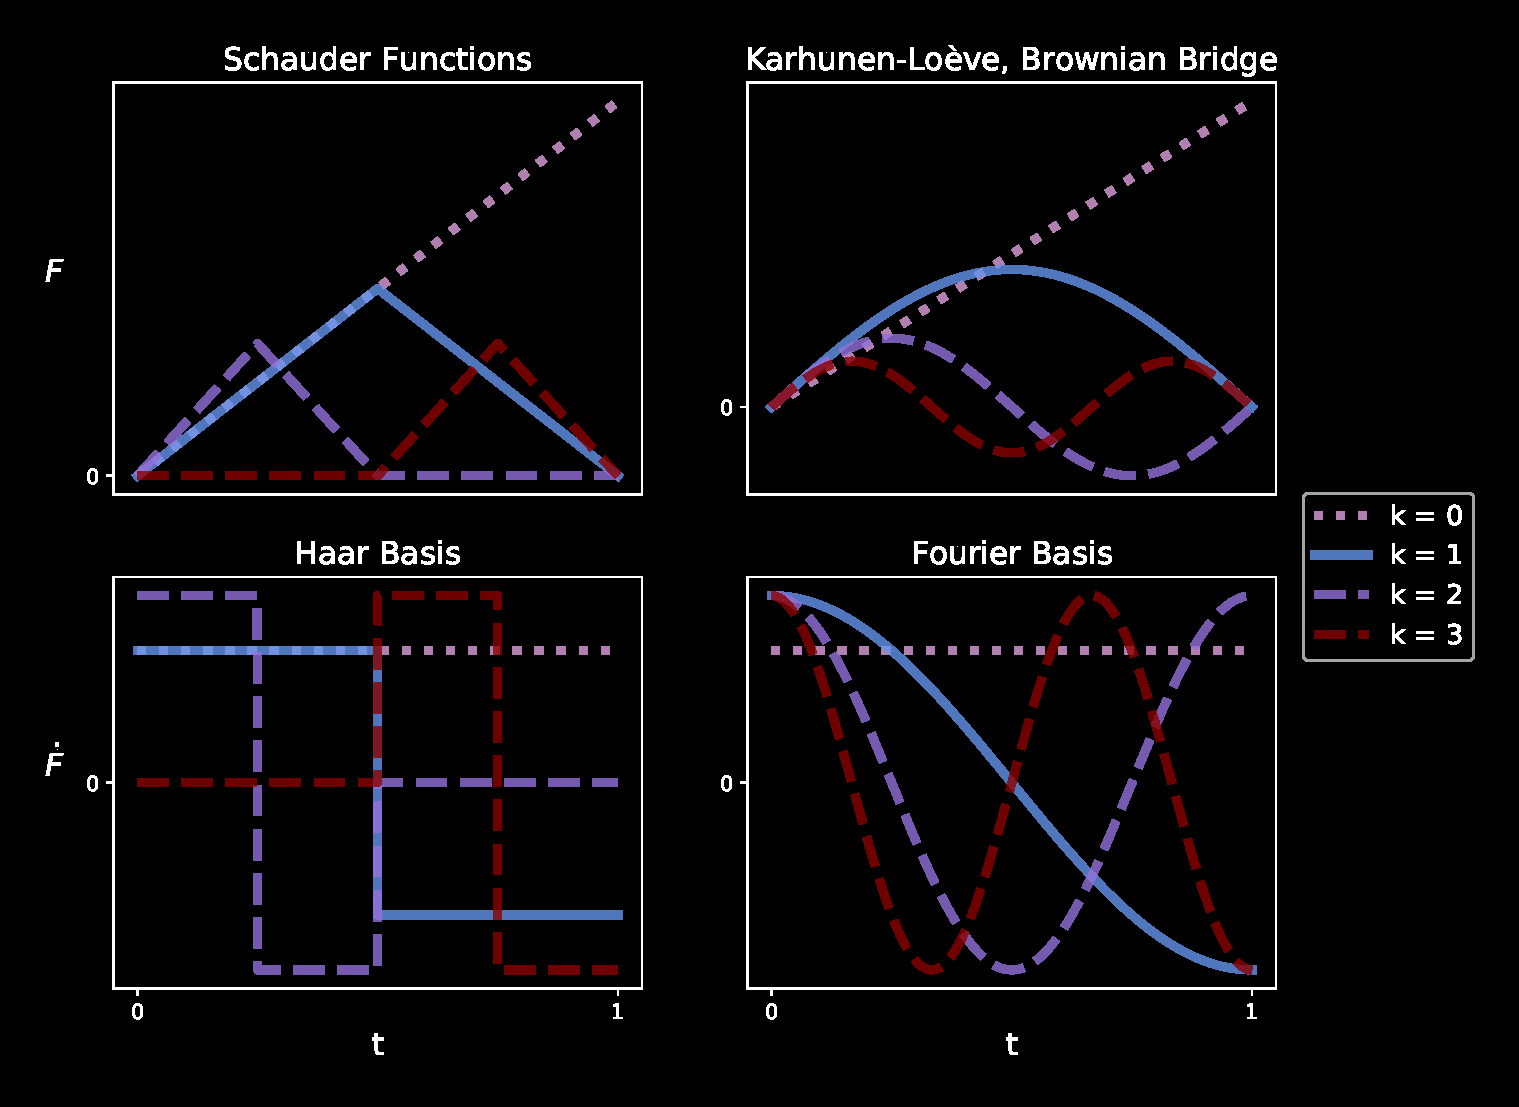
\includegraphics[scale = 0.35]{KL/Figures/LevyCieselski2.pdf}
    \label{fig:CMS}
\end{figure}

\begin{example}\label{ex:BBC}

A standard method to prove the existence of Brownian motion follows from the \text{Brownian bridge construction}. In short, it consists of a random superposition of triangular functions$-$the Schauder functions$-$obtained by integrating the Haar basis on $[0,1]$,
$$\dot{F}_{k,l}(t)=2^{k/2} \, \psi \left(2^{k}t-l\right),\quad 0 \le l \le 2^k,\quad t\in [0,1],$$
with the wavelet $\psi= (-1)^{ \mathds{1}_{[1/2, 1)}}$,  $\textnormal{supp}(\psi) = [0,1]$. It is easily seen that $\dot{F}_{k,l}$ as well as $F_{k,l}$ have support  
$[l/2^k,(l+1)/2^k]$, the $l-$th subinterval of the dyadic partition $\Pi_{k} = \{l/2^k\,|\, l = 0,\ldots,2^k\}$. 
The Schauder and Haar functions are illustrated on the left side of  \Cref{fig:CMS}.  Note that the total number of basis functions employed is $K = |\{(k,l) \,|\, 0 \le l \le 2^k , \, k=0,\ldots, \bar{K} \}| = 2^{\bar{K}+1}-1$ when considering all functions up to the $\bar{K}-$th dyadic partition. 
For Brownian motion, the approximation error is known \cite{Brown} and equal to  $\epsilon^{K,\frakF} = \frac{1}{6K}.$


\end{example}

\begin{example}\label{ex:cosine}
Let $(\dot{F})$ be the \text{cosine Fourier ONB}, i.e.
$\dot{F}_k(t) = \sqrt{2}\cos(\pi k t)$, $t \in [0,1]$. The anti-derivatives $F_k(t) = \sqrt{2}\,\frac{\sin(\pi k t)}{\pi k}$ turns out to correspond$-$up to a factor$-$to the Karhunen-Lo\`eve basis of the \text{Brownian bridge}. Indeed, recalling that $\kappa_X(s,t) = s\wedge t - st$ if $X$ is a Brownian bridge, we have for the ONB $\, \tilde{\frakF} = (\tilde{F}_k) = (\pi k \, F_k)$, 
\begin{align*}
    (\kappa_X(\cdot,t),\tilde{F}_k) 
    = \sqrt{2}\left[(1-t)\int_0^t s\, \sin(\pi k s) ds + t \int_t^1 (1-s)\sin(\pi k s) ds\right]
    = \sqrt{2}\, \frac{\sin(\pi k t)}{\pi^2 k^2},
\end{align*}
using integration by parts in the last equality. 
The eigenvalues  are therefore $(\lambda_k^{\tilde{\frakF}}) = (\frac{1}{\pi^2 k^2})$. 
The first elements of $\tilde{\frakF}$ and the Fourier cosine ONB are displayed on the right charts of  \Cref{fig:CMS}.
Following the same argument as in  \cref{ex:KLBM}, the (minimal) projection error onto $K$ basis functions is approximately equal to $\frac{1}{\pi^2 K}$. This is less than Brownian motion, as little more is known about a Brownian bridge; $\Q-$almost all trajectories return to the origin.

\end{example}

% \begin{figure}[H]
%     \centering
%     \includegraphics[scale = 0.4]{Figures/LevyCieselski.pdf}
%     \caption{Bases in the Cameron-Martin space. }
%     \label{fig:CMS}
% \end{figure}
 
 
 
 
 
 
 
\subsection{Signature and Legendre Polynomials}\label{sec:sigLegendre}
An alternative characterization of a path is available through the so-called \textit{signature}  \cite{Lyons}.  Roughly speaking, the signature extract  from a path an infinite-dimensional skeleton, where  each "bone" contains inherent information. 
We start off with a few definitions. 
A \textit{word} is a sequence  $\alpha = \alpha_1 ... \alpha_k$ of letters from the alphabet $\{0,1\}$. The length of $\alpha$ is denoted  by $l(\alpha)$. 
Moreover, we augment a path $X \in \Lambda$ with the time itself $t \mapsto t$  and   write 
$x^0_{t} = t$, $x^1_{t} = x_t$.  The words $0,1$ are therefore identified with the time $t$ and path $x$, respectively. 
The \textit{signature} in $\Lambda$ is here seen as  a collection  of functionals $\calS= \{\calS_{\alpha}: \Lambda \to \R\}$ such that $\calS_{\emptyset}(X_t) \equiv 1$ and 
$$\calS_{\alpha}(X_t) =
\int_{0}^{t} \int_{0}^{t_k} \cdots \int_{0}^{t_2} \circ \, dx^{\alpha_1}_{t_1} \cdots \circ dx^{\alpha_k}_{t_k}, \qquad l(\alpha)=k \ge 1,$$
     where  $\circ$ indicates Stratonovich integration.\footnote{When either the integrand or  integrator has bounded variation, the integral is in the  Riemann-Stieljes sense  and the symbol $\circ$ can be omitted. \vspace{2mm}} When referring to a specific path $X$, we shall call the sequence $(\calS_{\alpha}(X))$  the \textit{signature of $X$}. If $x_t\in \R^d$ with $d\ge 2$, then the alphabet becomes $\{0,1,\ldots,d\}$ and  the signature is  defined  analogously.  
The first signature functionals read
\begin{align*}
    \calS_{0}(X_t) &= \int_0^t d t_1 = t, &&\calS_{1}(X_t) = \int_0^t \circ \,d x_{t_1} = x_t - x_0,\\
  \calS_{00}(X_t) &= \int_0^t \int_0^{t_2} d t_1 d t_2 =\frac{t^2}{2}, &&\calS_{11}(X_t) = \int_0^t \int_0^{t_2}\circ \, d x_{t_1} \circ d x_{t_2}=\frac{(x_t-x_0)^2}{2},\\
  \calS_{10}(X_t) &= \int_0^t \int_0^{t_2} dx_{t_1}  d t_2 =\int_0^t (x_{s} - x_0) ds, &&\calS_{01}(X_t) = \int_0^t \int_0^{t_2} d t_1 d x_{t_2} =\int_0^t s \,dx_s.
\end{align*}
Keeping track of the passage of time  is crucial, as the signature would otherwise barely carry  information about the path. Indeed, notice that
$\calS_{\alpha}(X_t) = \frac{(x_t-x_0)^{k}}{k!}$ for  $\alpha =  1...1$, $l(\alpha)=k$ 
(as seen above for $k=1,2$) thus only the increment $x_t-x_0$ is known with the alphabet $\{1\}$. 
 
A property of the signature is that it uniquely characterizes a path, up to a  equivalence relation: two paths having same signature differ at most by a \textit{tree-like path} \cite{Hambly}, a specific type of loop.  
Hence, extending a path with time 
not only enriches the  signature  but also
ensures  injectivity  as $t\to x^0_t =t$ is increasing. 
This gives hope to reconstruct the (unique) path associated to a  signature sequence. This was investigated 
 by \citet{Geng}, where the author shows a 
geometric reconstruction using polygonal approximations for Brownian paths. 
We propose a simple algorithm, in connection with our discussion on Hilbert projections.\footnote{I thank Bruno Dupire for suggesting this interesting parallel.} 
For ease of presentation, assume $x_0=0$ and $T=1$. We first make the following observation. 

\begin{lemma}\label{lem:Legendre}
Let $\overleftarrow{X}$ denote the \textit{time reversed path}, i.e. $\overleftarrow{\ x_t} = x_{1-t}$ and 
introduce the words $\alpha^{(k)} :=10\ldots0\,$, $l(\alpha^{(k)})=k+2$, $k \ge 0$. 
Then $\calS_{\alpha^{(k)}} (\overleftarrow{X}_{\! 1})  = \frac{1}{k!}(X, m_k) $ where $m_k(t)=t^k$.
\end{lemma}
\begin{proof} First, observe that 
\begin{equation}\label{eq:100}
    \calS_{\alpha^{(k)}}(X_{t}) = \int_0^{t} x_s \frac{(t -s)^{k}}{k!}ds,\quad \forall \, t \in [0,1]. 
\end{equation}
Indeed for fixed $t\in [0,1]$ and  $k=0$, then $\calS_{\alpha^{(0)}}(X_t)=\calS_{10}(X_t) = \int_0^t x_sds$, which is $\eqref{eq:100}$. Now by induction on $k\ge 1$, uniformly on $[0,t]$,
\begin{align*}
  \calS_{\alpha^{(k)}}(X_t) = \int_0^t \calS_{\alpha^{(k-1)}}(X_u)du 
    = \int_0^t \int_0^u x_s \frac{(u -s)^{k-1}}{(k-1)!}ds\, du 
    = \int_0^t x_s \frac{(t -s)^{k}}{k!} ds.
\end{align*}
Now taking $t=1$ and $\overleftarrow{X}$ instead of $X$, we get
$
    \calS_{\alpha^{(k)}}(\overleftarrow{X}_{\! 1}) = \int_0^1 \overleftarrow{\ x_t}\frac{(1 -t)^{k}}{k!}dt =  \frac{1}{k!}(x,m_k).
$
\end{proof}

Essentially,  \Cref{lem:Legendre} states that the knowledge of $(\calS_{\alpha^{(k)}}(\overleftarrow{X}_{\! 1}))_{k\ge 0}$ is equivalent to the knowledge of the inner products of the path with the monomials. Since  also 
\begin{align*}
    \calS_{\alpha^{(k)}}(\overleftarrow{X}_{\! 1})
    &= (-1)^{k}\int_0^1 x_t \frac{((1-t)-1)^{k}}{k!}dt 
    %= (-1)^{k} \sum_{j=0}^k {k \choose j} \int_0^1 x_t \frac{(1-t)^{j}(-1)^{k-j}}{k!}dt \\
    = \sum_{j=0}^{k} \calS_{\alpha^{(j)}}(X_1) \frac{(-1)^{j}}{(k-j)!},
\end{align*}
the coefficients $(X,m_k)_{k\ge 0}$ can be retrieved from $(\calS_{\alpha^{(k)}}(X_1))_{k\ge 0}$ as well. 
To fall within the context of orthonormal projection, we transform the monomials into the (unique) polynomial ONB of $L^2([0,1])$. 
Let $(p_k)$ be the Legendre polynomials \cite{Szego}, forming an orthogonal basis of $L^2([-1,1])$. Then  consider the \textit{shifted Legendre polynomials},  $q_k(t) = p_k(2t-1),$  $t\in [0,1].$ 
We write 
$$q_k(t)= \sum_{j\le k} a_{k,j}t^j, \quad a_{k,j} = (-1)^{k+j} {k \choose j} {k + j \choose j},$$ with coefficients  derived for instance from  \textit{Rodrigues' formula} \cite[Section 4.3]{Szego}. The standardization $F_k :=  \frac{q_k}{\lVert q_k\rVert} = \sqrt{2k+1}q_k$ makes $\frakF = (F_k)$ an ONB of $L^2([0,1])$. This leads us to the following result. 
\begin{proposition}
If  $b_{k,j} := \sqrt{2k+1} j!\, a_{k,j}$ and $G_j(t) := \sum_{k= j}^K b_{k,j}\,  F_k(t)$, then 
\begin{equation}\label{eq:sigLeg}
    x^{K,\frakF}_t 
    = \sum_{k\le K} \xi_k F_k(t)
    =  \sum_{j \le K} \calS_{\alpha^{(j)}}(\overleftarrow{X_1})  G_j(t).
\end{equation}
\end{proposition}

\begin{proof}
 First, note that $(X,F_k) = \sum_{j\le k} a_{k,j}\, (X,m_j)$.   Using \cref{lem:Legendre}, we obtain 
$\xi_k = \sum_{j \le k} b_{k,j}\, \calS_{\alpha^{(j)}}(\overleftarrow{X_1})$. Hence,   $ x^{K,\frakF}_t   = \sum_{j \le K} \calS_{\alpha^{(j)}}(\overleftarrow{X_1})  G_j(t)$ with $(G_j)$ as in the statement.
\end{proof}
In summary, the signature elements $(\calS_{\alpha^{(k)}})_{k\le K}$ generate the $L^2([0,1])$ products of the path with the monomials$-$and in turn, with the Legendre polynomials$-$from which the projected path $X^{K,\frakF} $ becomes available. 
We can therefore retrieve $X$ by letting $K\to \infty$. Note that this reconstruction  works for multidimensional paths as well, as we can apply the procedure to each component  $i=1,\ldots,d$ with the words
$\alpha^{(i,k)} :=i 0\ldots0$, $l(\alpha^{(i,k)}) = k+2$, $k \ge 0$.  
We finish this section by computing the projection error of $\eqref{eq:sigLeg}$ when $X$ is Brownian motion. Recalling that $\kappa_X(s,t) = s \wedge t$,  a  simple calculation gives 
$$\lambda_k^{\frakF} = \E^{\Q}[\xi_k^2] = 2 \int_{0}^1 \int_{0}^t s  F_k(s)dsF_k(t)dt = 2 (2k+1)\sum_{i,j \le k} \frac{a_{k,j}\ a_{k,i}}{(j+2)(i+j+3)}.
%(-1)^{k+j} {k \choose j} {k + j \choose j}
$$
 
The first values are given by $(\lambda^{\frakF}_k)_{k=0}^3 = (\frac{1}{3},\frac{1}{10}, \frac{1}{42}, \frac{1}{90})$ from which we  conjecture that $\lambda^{\frakF}_k = \frac{1}{(2k+3)(4k-2)}$ for all $k\ge 1$. This is supported by the fact that $\lambda^{\frakF}_k$ must be  rational numbers as $a_{k,j}\in \Z$ for all $k,j$ and 
$$\sum_{k=0}^K  \lambda^{\frakF}_k = \frac{1}{3} + \frac{1}{8} \sum_{k=1}^K  \left( \frac{1}{2k-1}-\frac{1}{2k+3} \right) = \frac{1}{2} - \frac{K+1}{(2K+3)(4K+2)} \xrightarrow{K \uparrow \infty} \frac{1}{2},$$ coinciding with the total variance of Brownian motion on $[0,1]$.  
Thus, the approximation error reads  $\epsilon^{K, \frakF} =\frac{K+1}{(2K+3)(4K+2)} = \calO(\frac{1}{8K})$, which is of course larger than the Karhunen-Loève basis but smaller than the Brownian Bridge construction (\cref{ex:BBC}). Note that polynomial ONB's may well be optimal if the approximation criterion is modified. In \cite{Foster}, the authors show that in the weighted Hilbert space $L^2([0,1],\mu)$, $\mu(dt) = \frac{dt}{t(1-t)}$, the Karhunen-Loève basis of the Brownian bridge is formed by the anti-derivatives of the Legendre polynomials. Although the construction is different, it  is also curiously related to the signature elements $(\calS_{\alpha^{(k)}})$; see  Theorem 2.3 and  2.4 in \cite{Foster}.

%In \cite{Foster}, the authors show that representation of Brownian motion with polynomials arising from the Karhunen-Loève expansion of the Brownian bridge in the weighted Hilbert space $L^2([0,1],\mu)$, $\mu(dt) = \frac{dt}{t(1-t)}$ is .  Therefore, a polynomial ONB may well be optimal if the approximation criterion is modified. Although the polynomial expansion is different, the same signature elements appear;  in \cite{Foster}; .

\begin{remark}
Note that the approximation in $\eqref{eq:sigLeg}$ may be improved by adding other elements of the  signature, especially those that are \textit{nonlinear} in $X$, e.g. $\calS_{110}(X_t) = \frac{1}{2}\int_0^t x^2_s ds $.  We postpone this discussion to  \Cref{sec:sigFunc} when projecting  running functionals.
\end{remark} 
 
 \begin{figure}[t]
    \centering
    \caption{Projected paths with $K=8\,$ basis elements. }
    \vspace{-2mm}
    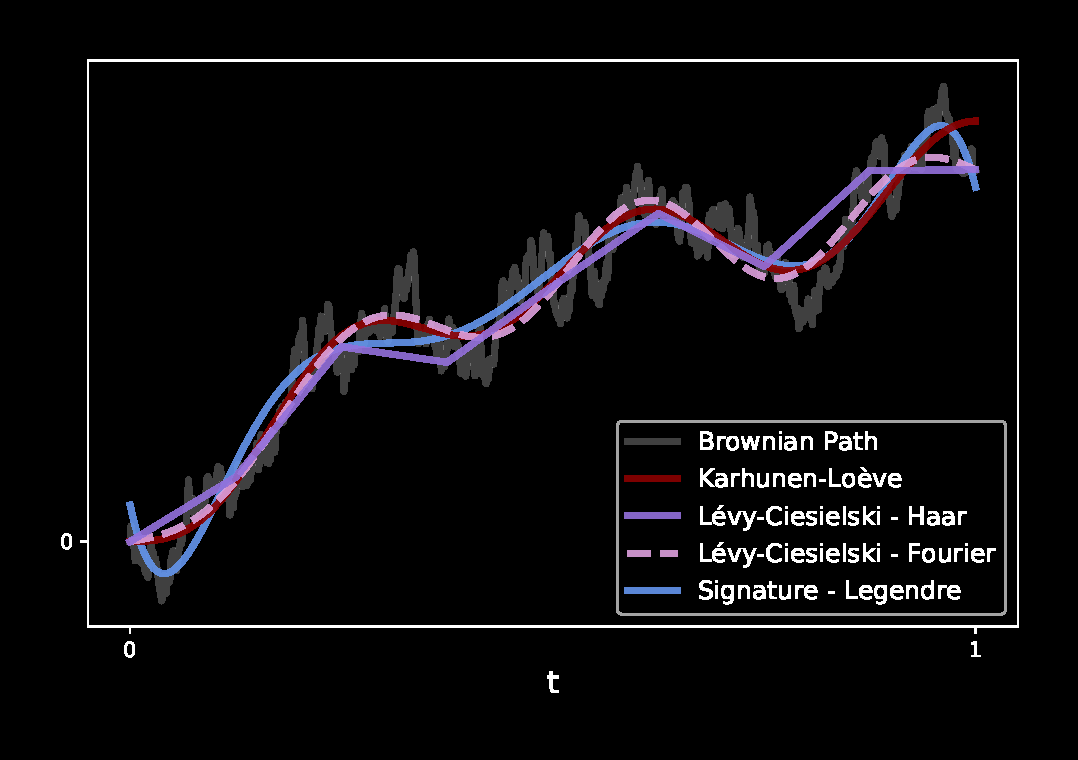
\includegraphics[scale = 0.45
    ]{KL/Figures/ProjPath.pdf}
    \label{fig:projPath}
\end{figure}
 \subsection{Numerical Results}\label{sec:numResultX}

We concentrate our experiments on Brownian trajectories.  
First, we illustrate %visualize and compare 
the  path  approximations seen earlier (Karhuhen-Loève, L\'evy-Cieselski, Signature).
Figure \ref{fig:projPath} displays the projections using $K=8$ basis elements. We naturally notice similarities between the Karhunen-Loève transform and the L\'evy-Cieselski construction with Fourier cosines, both 
obtained by superposing trigonometric functions.

Let us gauge the accuracy of the above approximations for Brownian trajectories, in terms of (i) 
    $\epsilon^{K,\frakF}$ and (ii) variance explained 
    $ \vartheta^{K,\frakF} := \frac{\lVert X^{K,\frakF}  \rVert^2_{*}}{\left \lVert X \right \rVert^2_{*}}.$ 
To compute (i), (ii) and the coefficients $(X,F_k)_{\calH}$, we discretize the interval $[0,1]$ a regular partition made of $N = 10^4$ subintervals. 
\Cref{fig:Error_VarExp} displays the evolution of $\epsilon^{K,\frakF}$, $\vartheta^{K,\frakF}$ for $K\in \{1,\ldots,128\}$. The Karhunen-Lo\`eve expansion clearly dominates the other projections, although being asymptotically equivalent to the L\'evy-Cieselski construction with Fourier cosine basis. Besides, the $L^2(\mathbb{Q} \, \otimes \, dt)$ convergence of the Brownian bridge construction (L\'evy-Cieselski with Haar basis) is non-monotonic. Indeed, a bump appears until a full cycle of the dyadic partition is completed. 
Lastly, the slopes in the log-log convergence plot  (left chart of \Cref{fig:Error_VarExp}) 
are roughly equal to $-1$. Put differently,  the squared approximation error is of order $\calO(\frac{1}{K})$, confirming our findings from the  above examples.

\begin{figure}[t]
    \centering
    \caption{$L^2(\mathbb{Q} \, \otimes \, dt)$ error and variance explained.}
    \vspace{-2mm}
    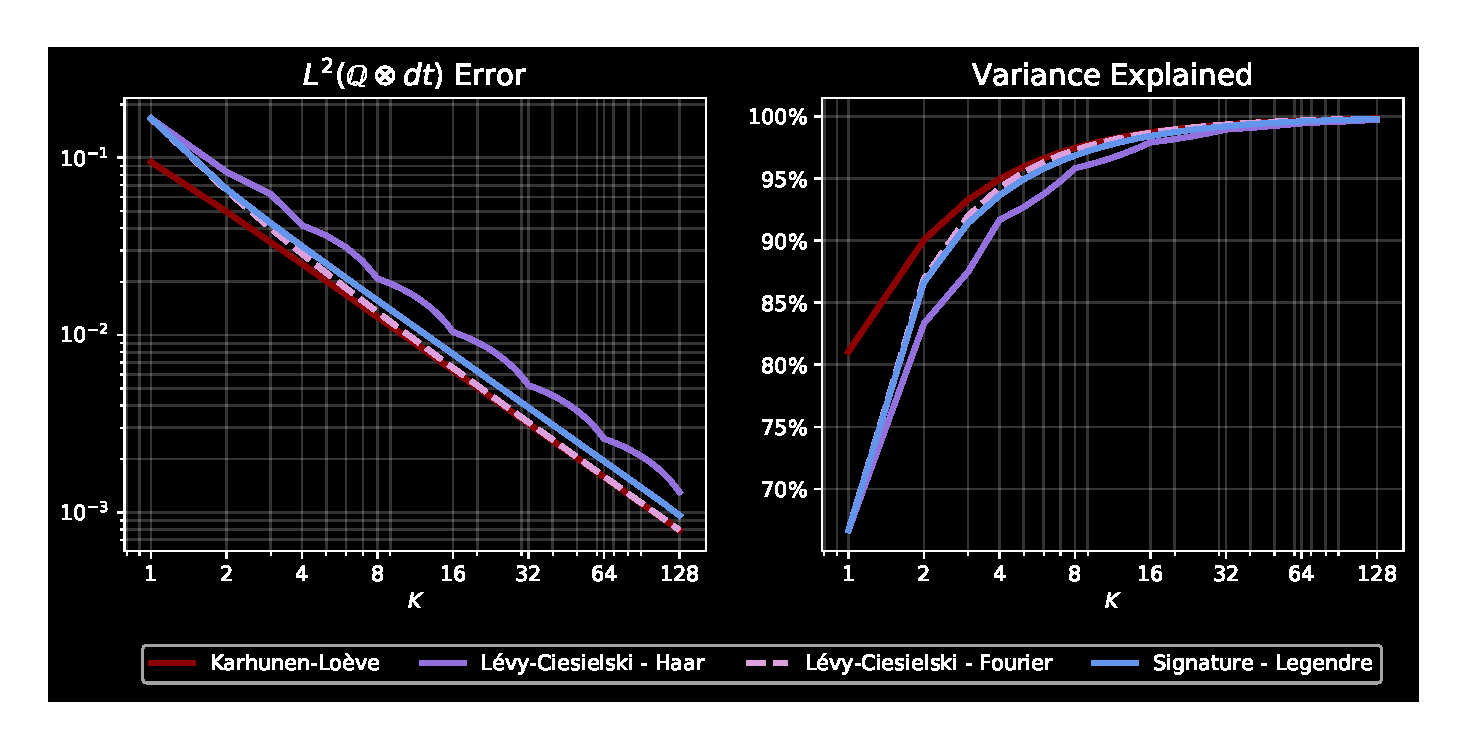
\includegraphics[scale = 0.45]{KL/Figures/Err_VarExp.pdf}
    \label{fig:Error_VarExp}
\end{figure}
 
\section{Projection of Functionals}
\label{sec:funcApprox}
In  \Cref{sec:pathApprox}, we unveiled two ways to approximate exotic payoffs $\varphi = h\circ f$, namely by projecting the original path $X$ or $Y = f(X)$ directly.  If $\pi^{K,\frakF}$ denotes as before the projection map onto a Hilbert space $\calH$, we can therefore write $\varphi^{K,\frakF} := h\circ f^{K,\frakF}$, where either $f^{K,\frakF} = f \circ \pi^{K,\frakF}$ (functional of projected path)
or $f^{K,\frakF} = \pi^{K,\frakF} \circ f$ (projected functional). 
% This implies that the transformed path is projected  we can either take the image of the projected path  $(Y^{K,\frakF} = (\pi^{K,\frakF} \circ f)(X))$ or project $f(X)$ directly  $(Y^{K,\frakF} = (\pi^{K,\frakF} \circ f)(X))$. 
% This consists of taking the image of a projected path through the functional, namely $Y^{K,\frakF} =  f(X^{K,\frakF})$. 
We shall see in  \Cref{ssec: numResult} that the former is suboptimal. 
Although not so problematic for functionals capturing global features of a path, local path characteristics (e.g. running maximum) will typically be grossly estimated. Indeed, projecting a path first erases most of its microstructure. 
We thus favor the second option ($f^{K,\frakF} = \pi^{K,\frakF} \circ f$), which consists of replacing $X$ by $Y$ in $\eqref{eq:proj}$. Let us now focus on $\calH = L^2([0,T])$ and demonstrate how to compute the Karhunen-Loève basis of $Y$. 



\subsection{Karhunen-Loève Expansion of Functionals}



Assume that $Y \in L^2([0,T]) \cap \Lambda_T$ has  zero mean (otherwise, see \cref{rem:center}).   \cref{thm:KL} suggests to set  $\frakF$  equal to the eigenfunctions of  $\kappa_Y(s,t) = (y_s,y_t)_{L^2(\Q)}$. Optimality comes, however,  at the cost of explicitizing $\frakF$. We proceed as follows: take a regular partition $\Pi_N = \{t_n = n\, \delta t\, |\, n=0,\ldots,N\}$, $ \delta t =\frac{T}{N}$ and compute the kernel matrix $\kappa^{N}_Y = (\kappa_Y(t_n,t_m))_{0 \le n,m \le N}$. When $\kappa_Y$ does not admit a  closed-form expression, $\kappa^{N}_Y$ is replaced by the sample covariance matrix using simulated paths for $Y$. The eigenfunctions thus become eigenvectors and solve the systems\footnote{In  $\eqref{eq:eigendecomp}$,  $\sum"$ means that the first and last summand are halved, i.e. the trapezoidal rule is used to compute  $(\kappa_Y(\cdot,t), F_k)$. Another approach, known as Nyström's method  \cite{reinhardt} consists of   employing a Gaussian quadrature scheme instead.  
However, for large $N$,  we haven't observed any improvement 
and thus favor the more convenient discretization in  $\eqref{eq:eigendecomp}$.}
\vspace{-1mm}
\begin{equation}\label{eq:eigendecomp}
        \sum_{t_n\in  \Pi_N}\!\!" \, \kappa^{N}_{Y}(t_n,t_m) F_{k}(t_n)  \delta t = \lambda^{\frakF}_{k}\,  F_{k}(t_m), \quad t_m\in \Pi_N, \quad k=0,...,N.
\end{equation}
\vspace{-3mm}

 This is a simple eigenvalue problem so  all pairs $(F_k,\lambda_k^{\frakF})$ can be  computed in one go. Let us proceed with two examples where  $T=1$ and $\Q=$ Wiener measure throughout.

\begin{figure}[t]
    \centering
    \caption{Running maximum functional for two trajectories.}
    \vspace{-2mm}
    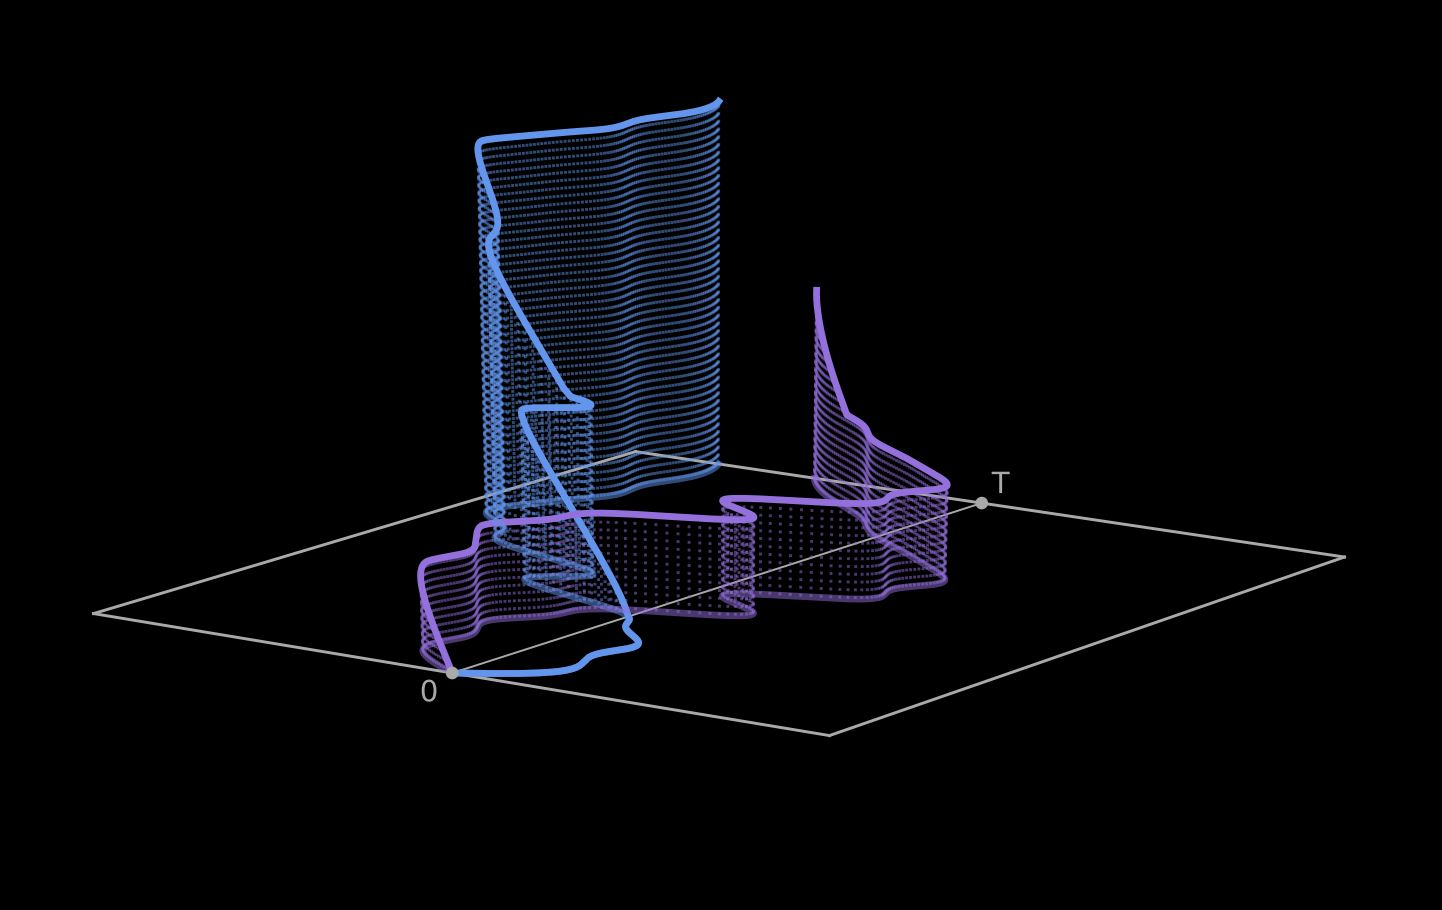
\includegraphics[scale =0.22]{KL/Figures/MaxDouble.JPG}
    %
    \label{fig:max3D}
\end{figure}



%========== Time Average and Integral ===========%
\begin{example} \label{ex:timeIntAvg}
 Consider  the time integral and average of a Brownian path, 
$y_t = 
f(X_t) = \int_0^t x_s\, ds, \ \bar{y}_{t}= 
\bar{f}(X_t) = \frac{1}{t}f(X_t). $
These are clearly centered processes and their covariance kernels of can be found explicitly. Starting with $Y$, 
$$\kappa_{Y}(s,t) =  \left(\int_0^s x_r dr,\int_0^t x_u du \right)_{L^2(\Q)} \overset{\textnormal{Fubini}}{=} \int_0^s\int_0^t \kappa_X(r,u) dr du.$$
A straightforward calculation gives
$\kappa_{Y}(s,t)  = \frac{s^2 t}{2} - \frac{s^3}{6}, \, s\le t.$
%\textbf{Moreover, it is straightforward to show that the eigenvalues are the square of the eigenvalues of Brownian (see Example \ref{ex:KLBM}).}
The covariance function of the time average follows immediately, namely
$\kappa_{\bar{Y}}(s,t)   = \frac{s}{2} -\frac{s^2}{6t}.$
We display in  \Cref{fig:AvgK,fig:IntK} the covariance kernel (top) and first eigenfunctions (bottom) of $f$ and $\bar{f}$, respectively.
The dashed lines in the top panels  are the eigenfunctions of the original (Brownian) path. Note the wider range in the eigenfunctions $F_1,F_2$ for $\bar{f}(X)$ compared to the integrated path for small $t$.  This might come from the greater fluctuations of the time average at inception. 

\end{example}
%========== Maximum ===========%
\begin{example} Consider the running maximum  functional $y_t= 
f(X_t) = \max_{0 \le s \le t} x_s$.  \Cref{fig:max3D} provides an illustration in the $(t,X,Y)$ plane. The mean function is in this case non-zero and$-$using, e.g., the reflection principle$-$given by $\E^{\Q}[y_t] = \sqrt{\frac{2}{\pi} t}$. The covariance kernel admits an explicit yet complicated expression \cite{Benichou}, 
$$\kappa_Y(s,t) = \frac{s}{2} + \frac{\sqrt{s(t-s)}-2\sqrt{st} + t \arcsin(\sqrt{s/t})}{\pi}, \quad s \le t.$$
\Cref{fig:MaxK} displays the covariance kernel (top) and first eigenfunctions (bottom). The latter turns out to be quite close to the eigenfunctions of Brownian motion. 

\end{example}



\begin{figure}[t]%[H]
%\centering
\caption{Covariance kernels (top) and eigenfunctions (bottom).}
\vspace{-4mm}
\begin{subfigure}[b]{0.32\textwidth}
    \centering
    \caption{Time average}
    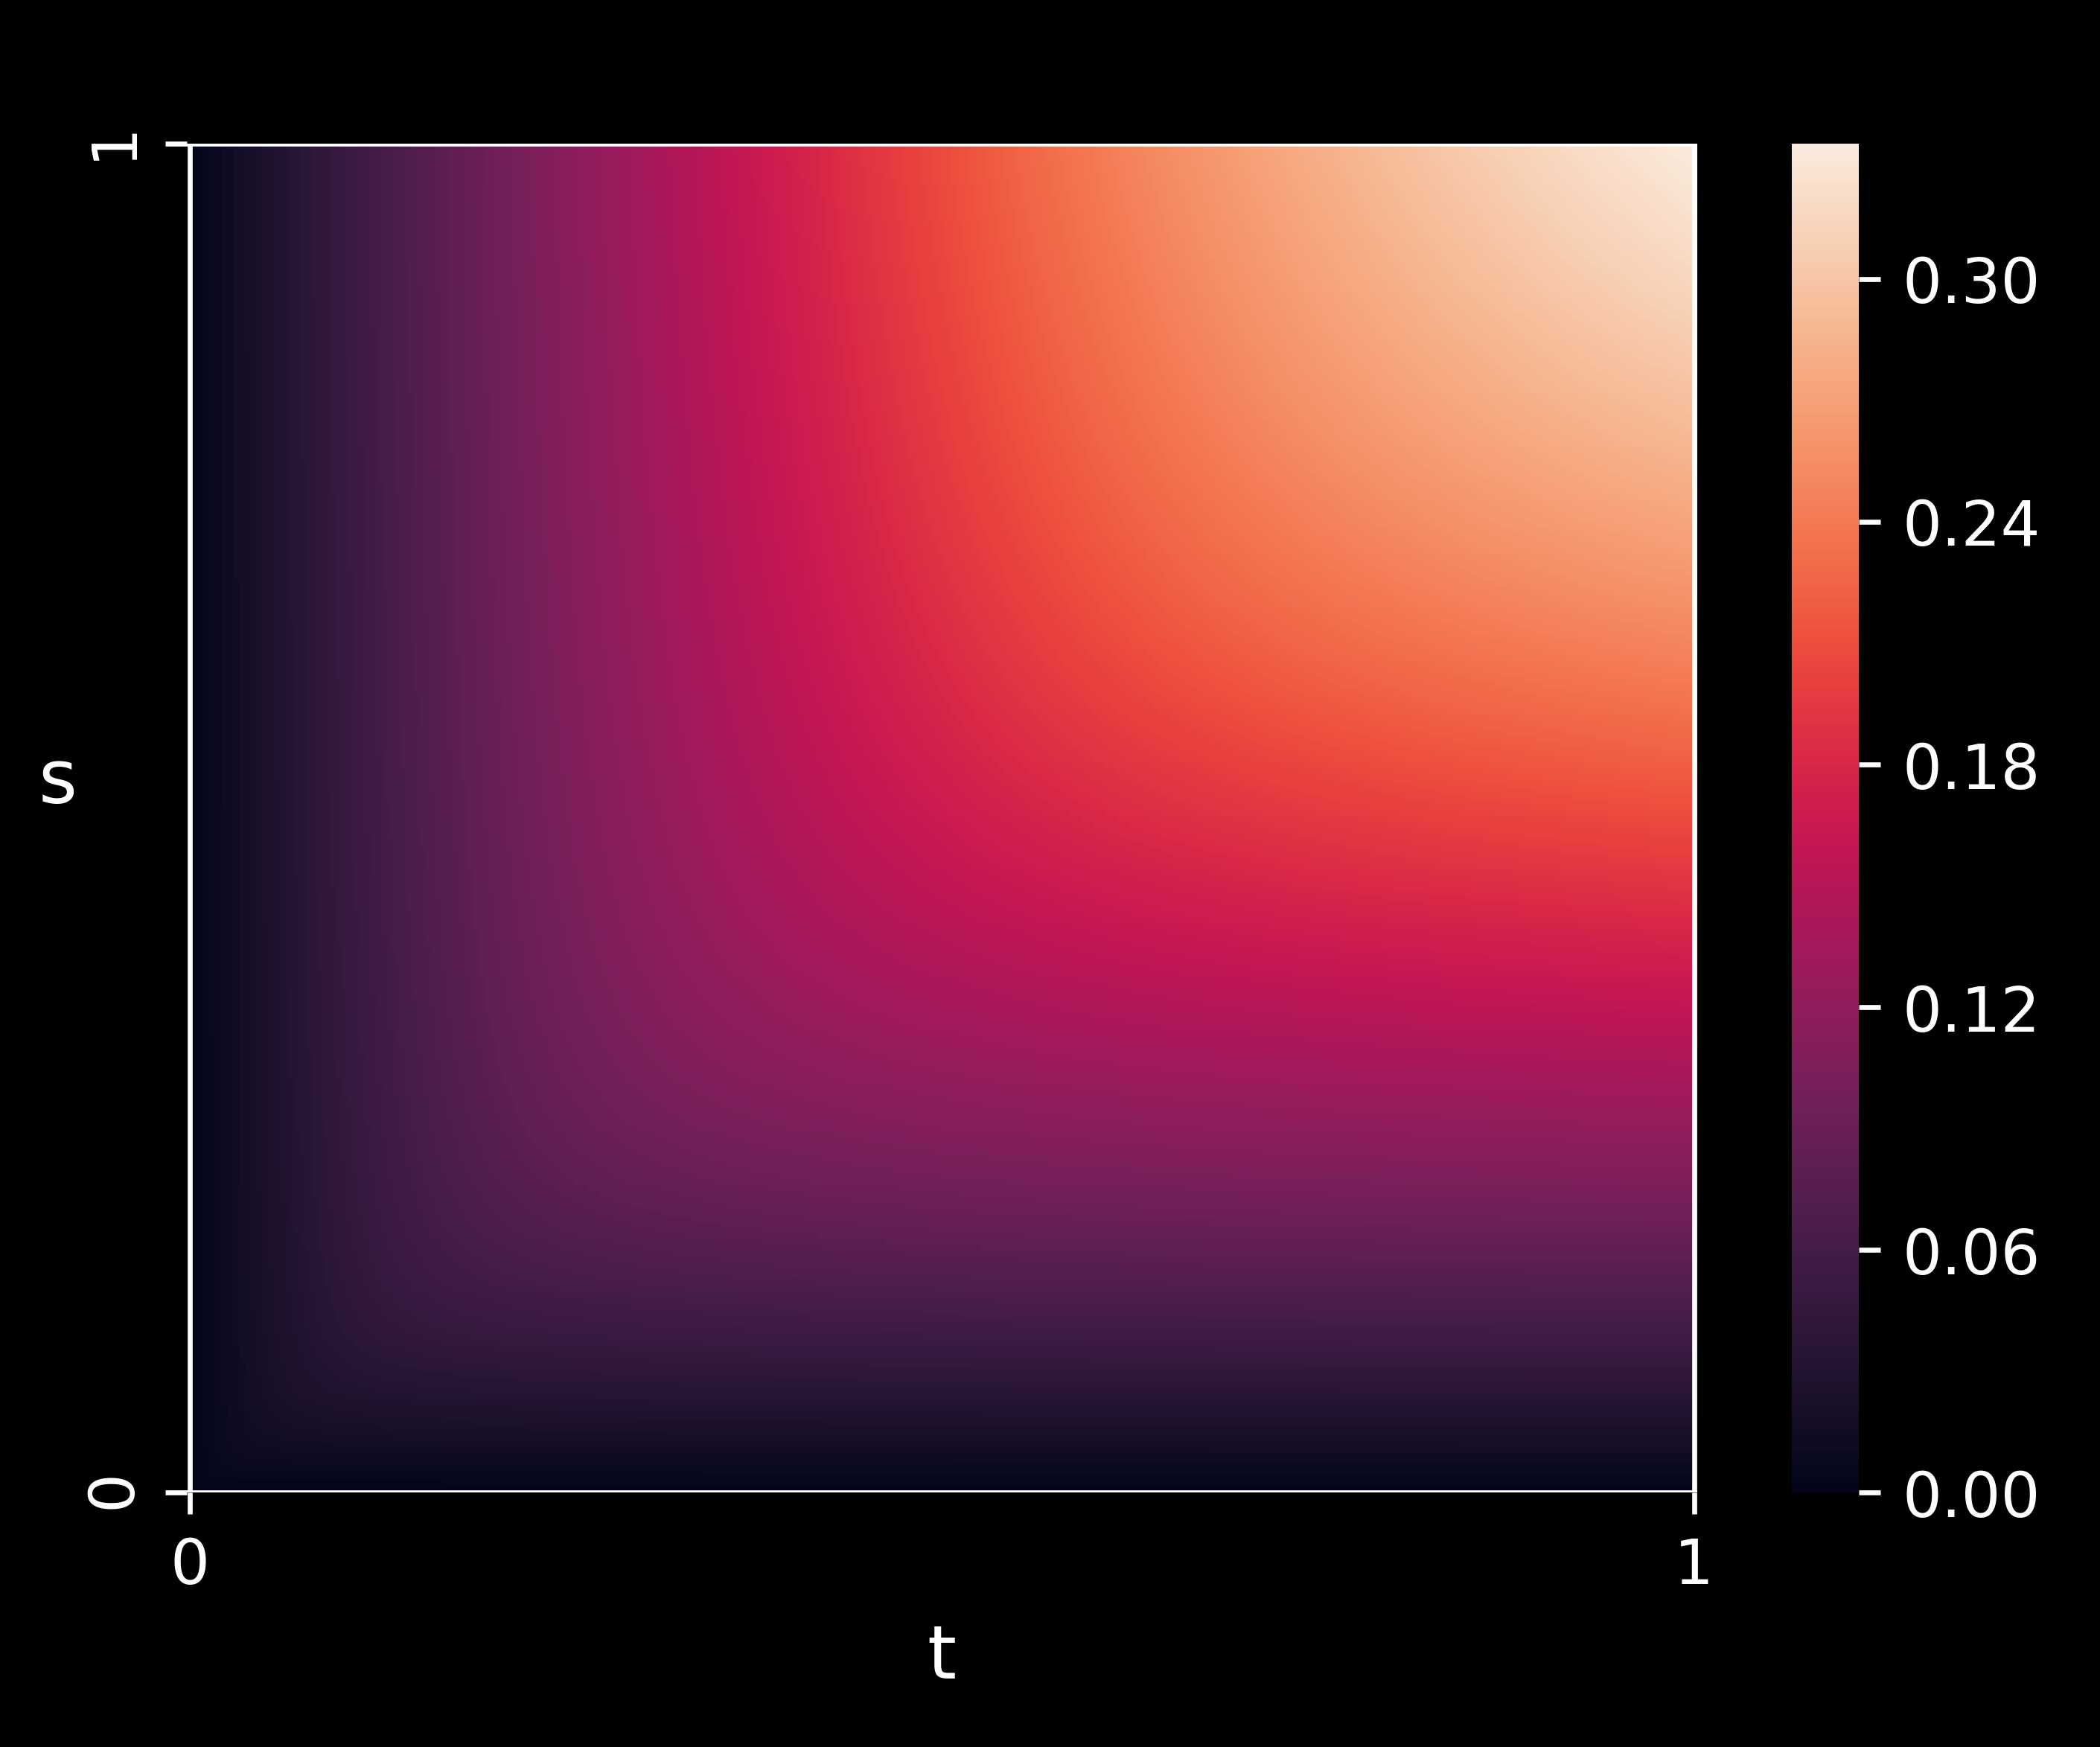
\includegraphics[scale =0.38]{KL/Figures/KLAverageKernel.png}
    \label{fig:AvgK}
\end{subfigure}
\begin{subfigure}[b]{0.32\textwidth}
    \centering
    \caption{Time integral}
    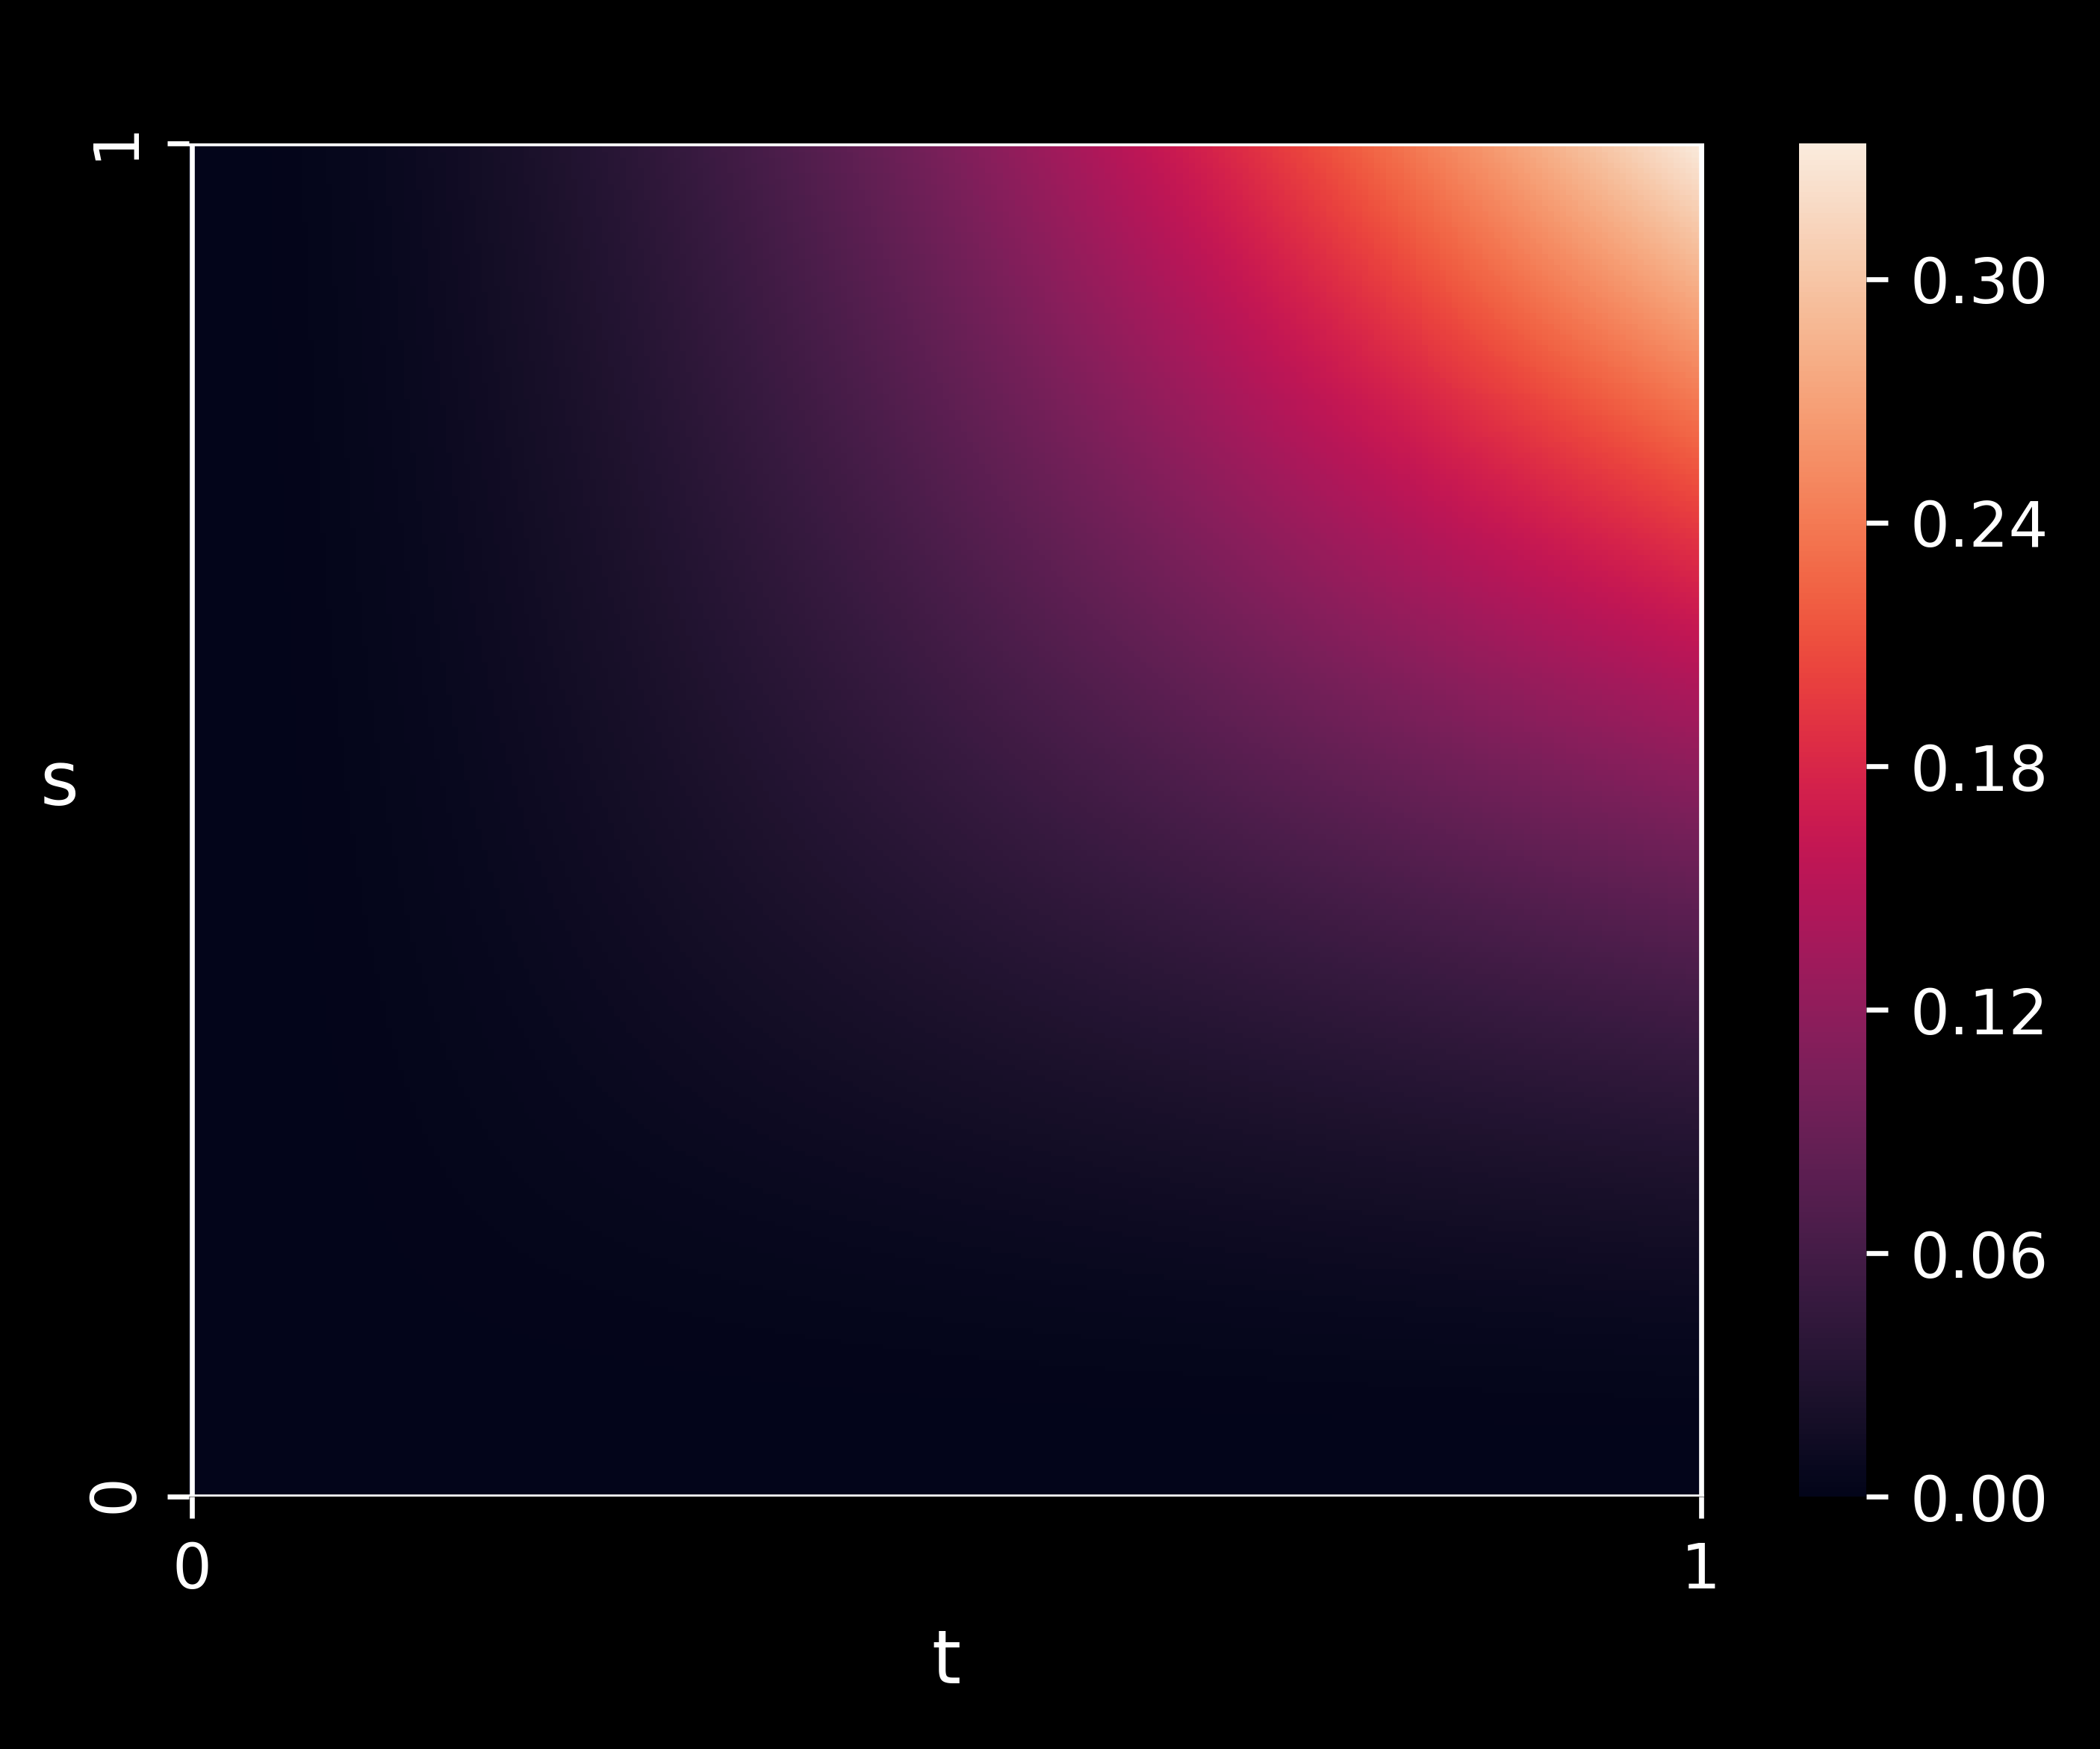
\includegraphics[scale =0.38]{KL/Figures/KLIntegralKernel.png}
    \label{fig:IntK}
\end{subfigure}
\begin{subfigure}[b]{0.32\textwidth}
    \centering
    \caption{Running maximum}
    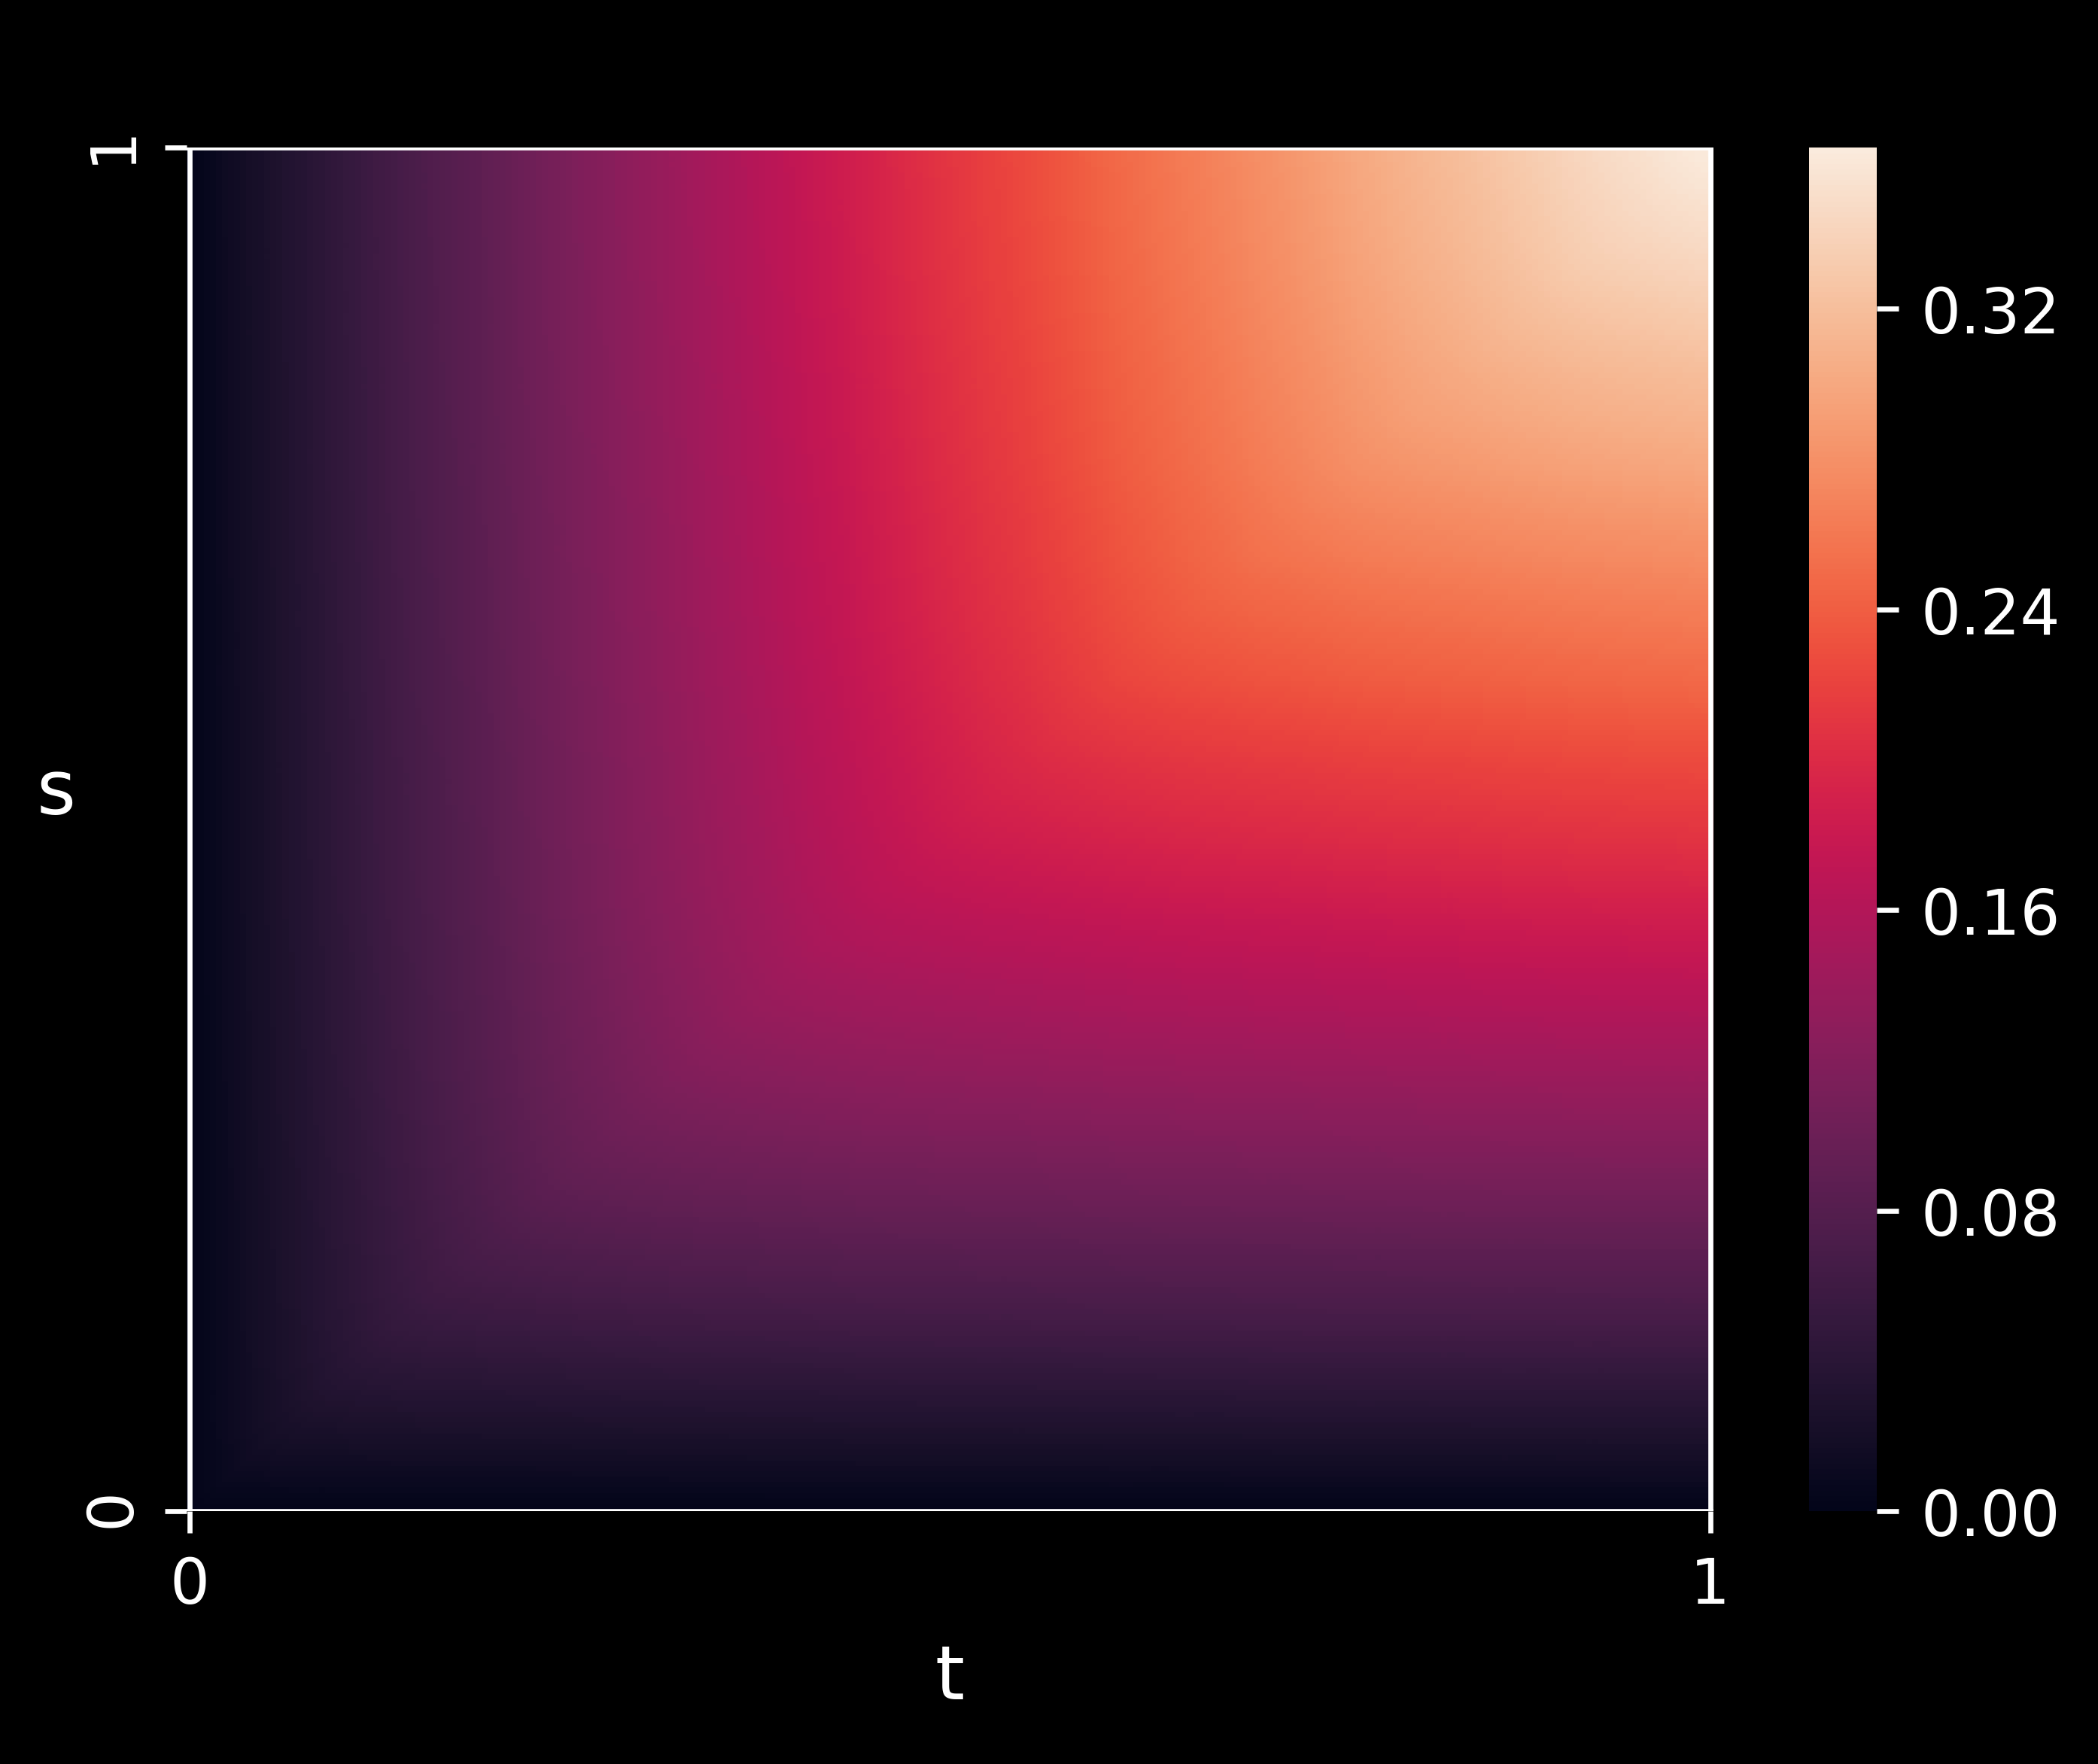
\includegraphics[scale =0.38]{KL/Figures/KLMaximumKernel.png}
    \label{fig:MaxK}
\end{subfigure}
\vspace{2mm}

%\centering
\begin{subfigure}[b]{0.32\textwidth}
    \centering
    %\caption{Time average}
    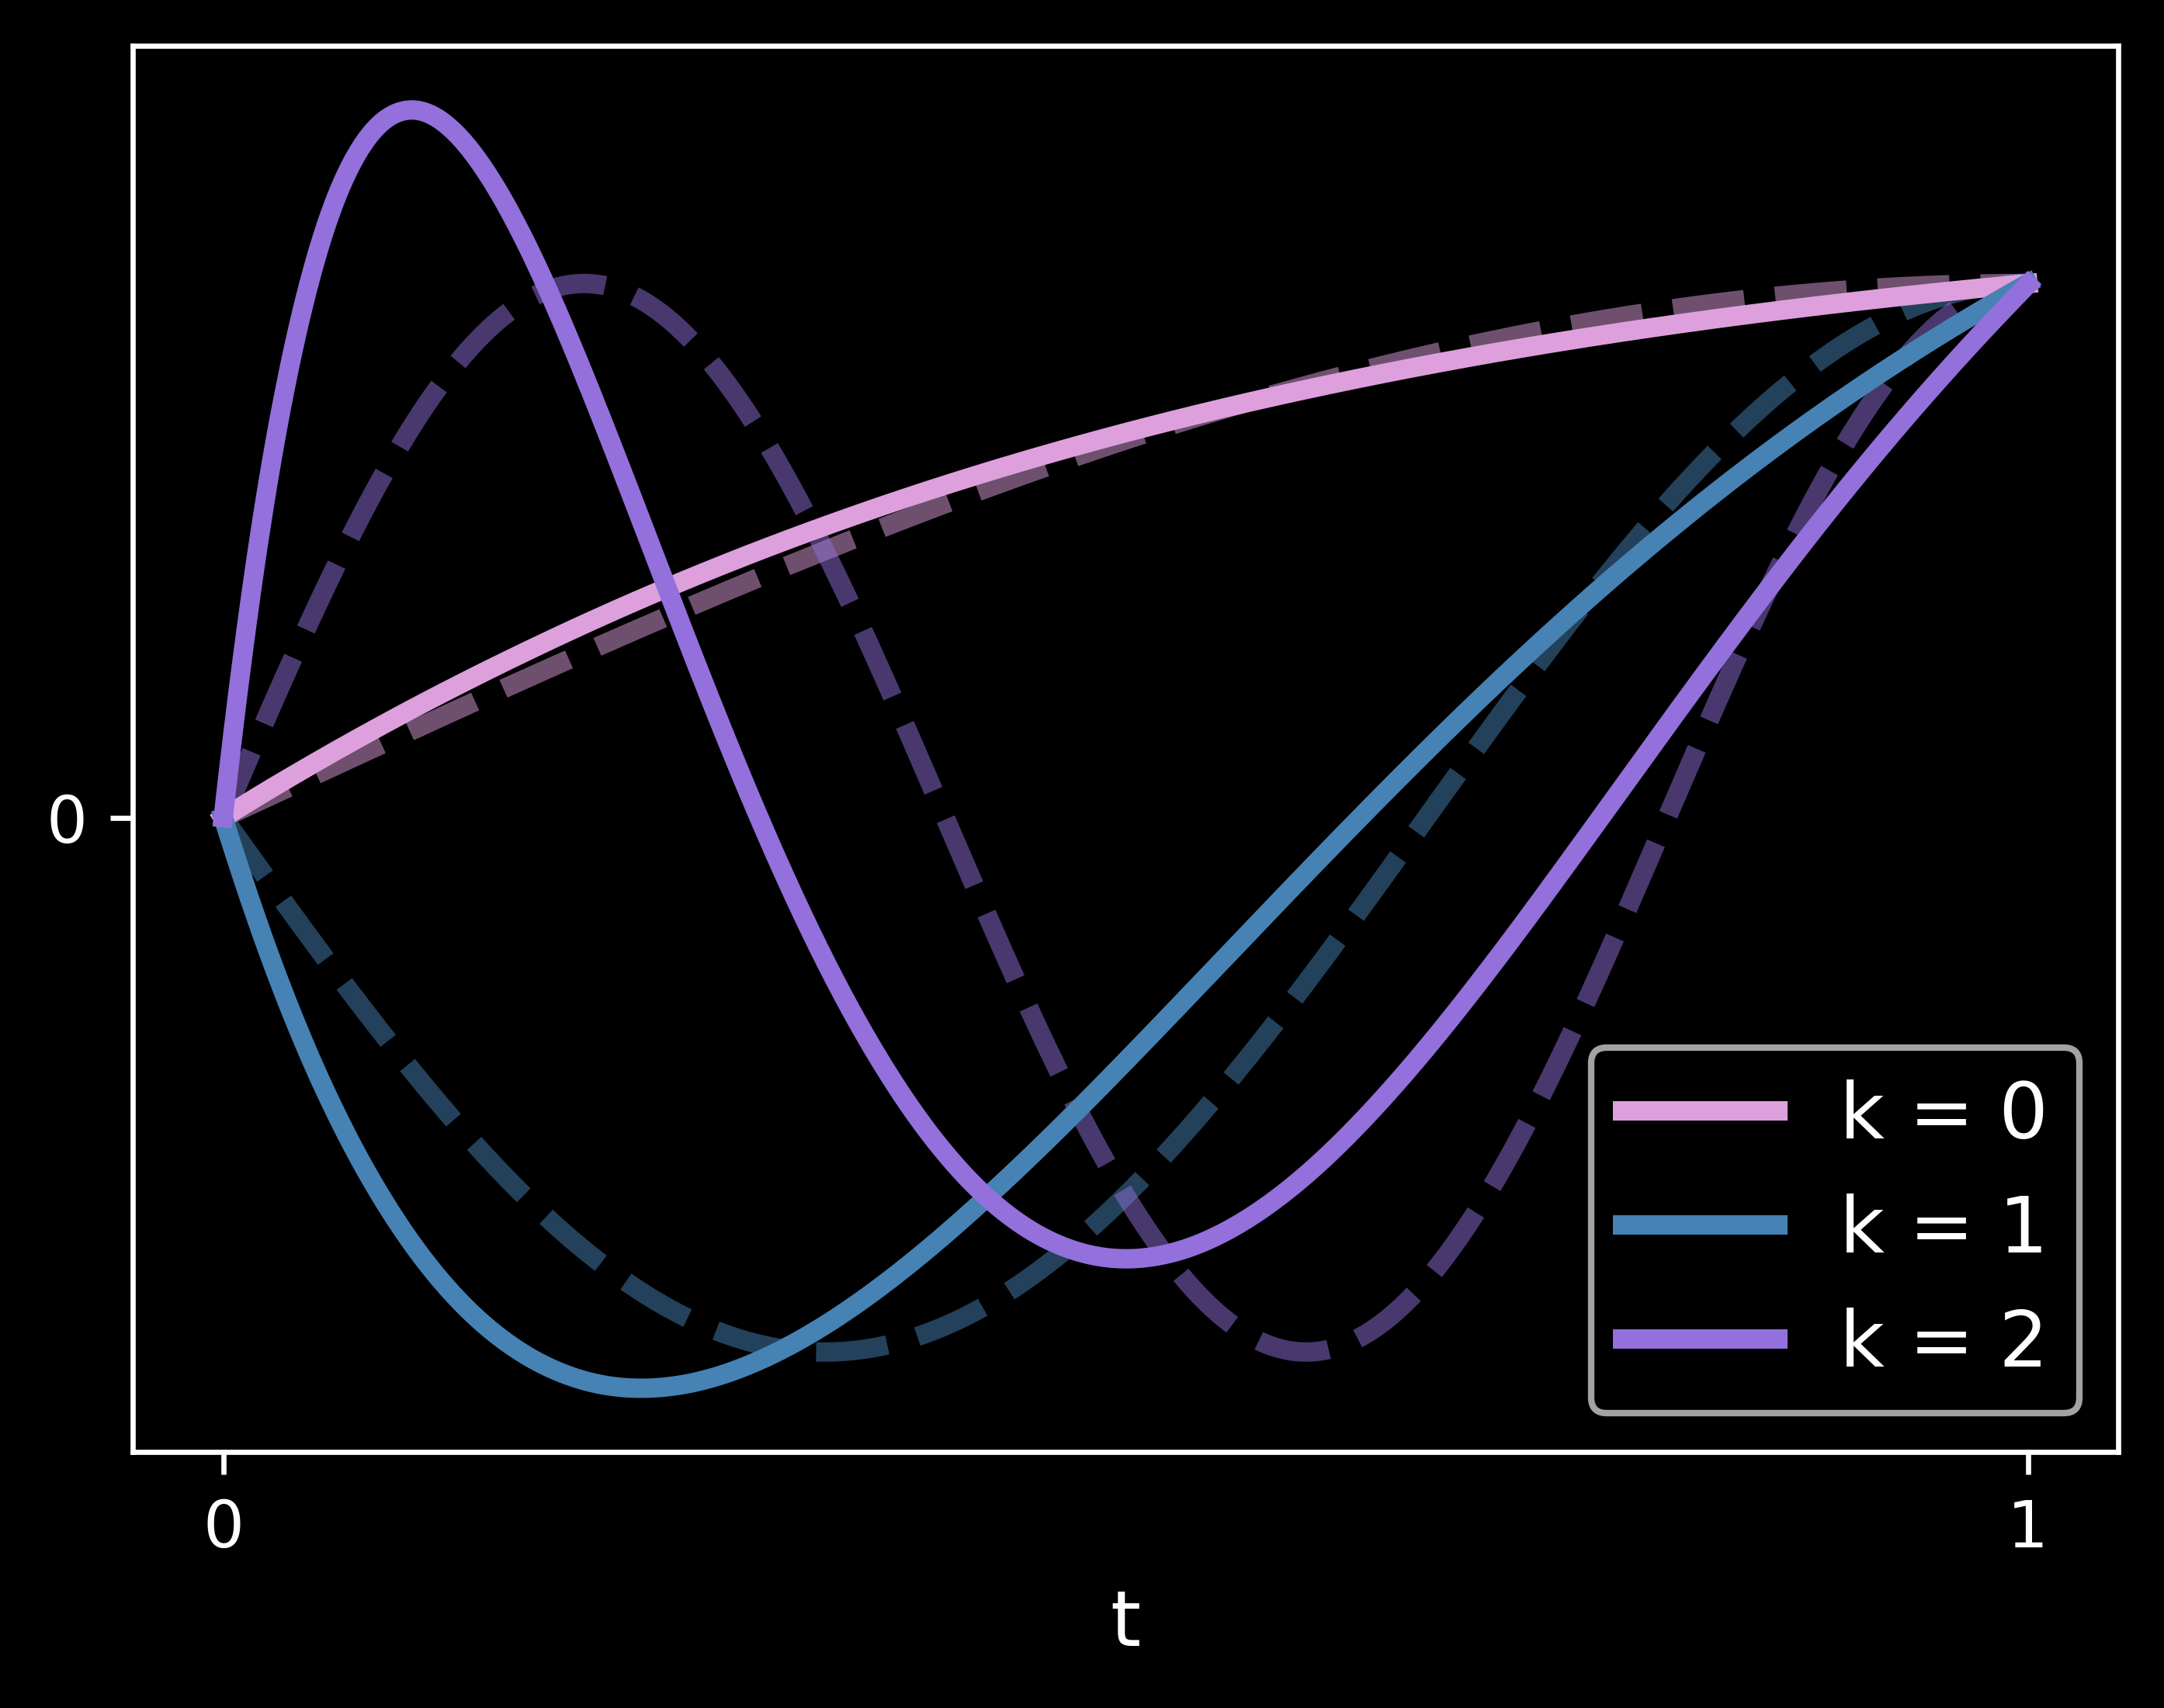
\includegraphics[scale =0.385]{KL/Figures/KLAsian.png}
\end{subfigure}
\begin{subfigure}[b]{0.32\textwidth}
    \centering
    %\caption{Time integral}
    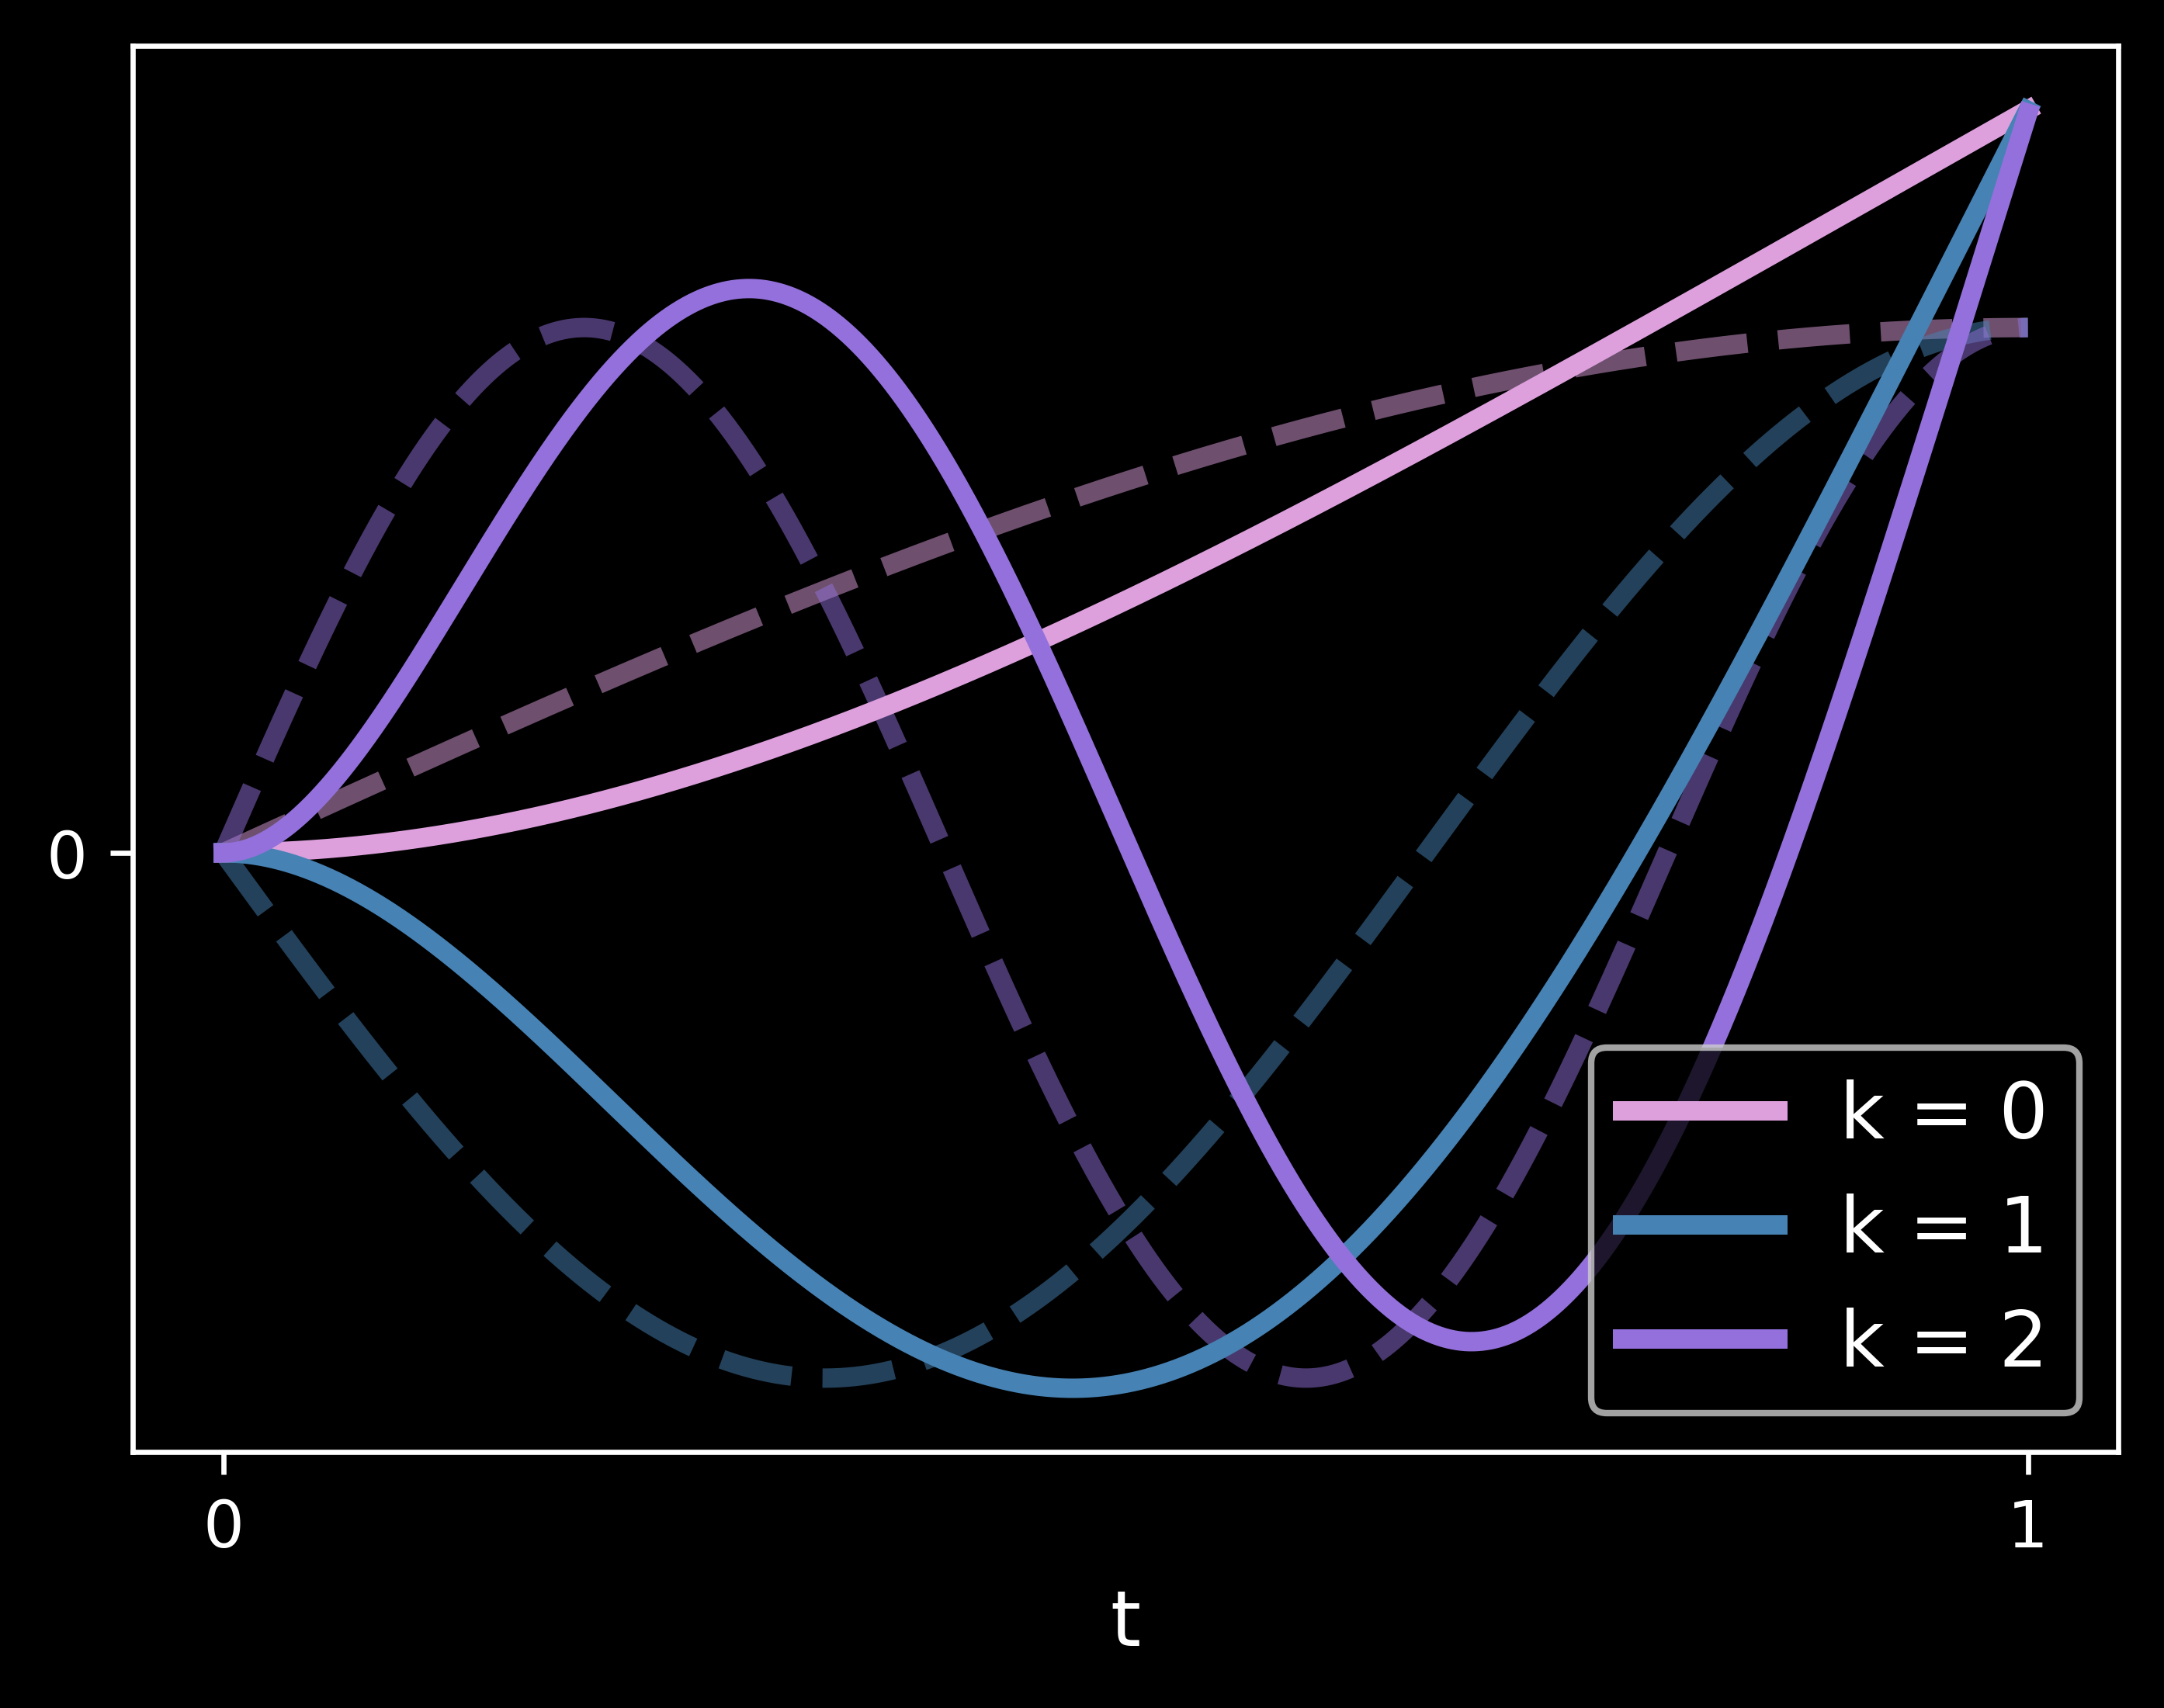
\includegraphics[scale =0.385]{KL/Figures/KLIntegral.png}
\end{subfigure}
\begin{subfigure}[b]{0.32\textwidth}
    \centering
    %\caption{Time integral}
    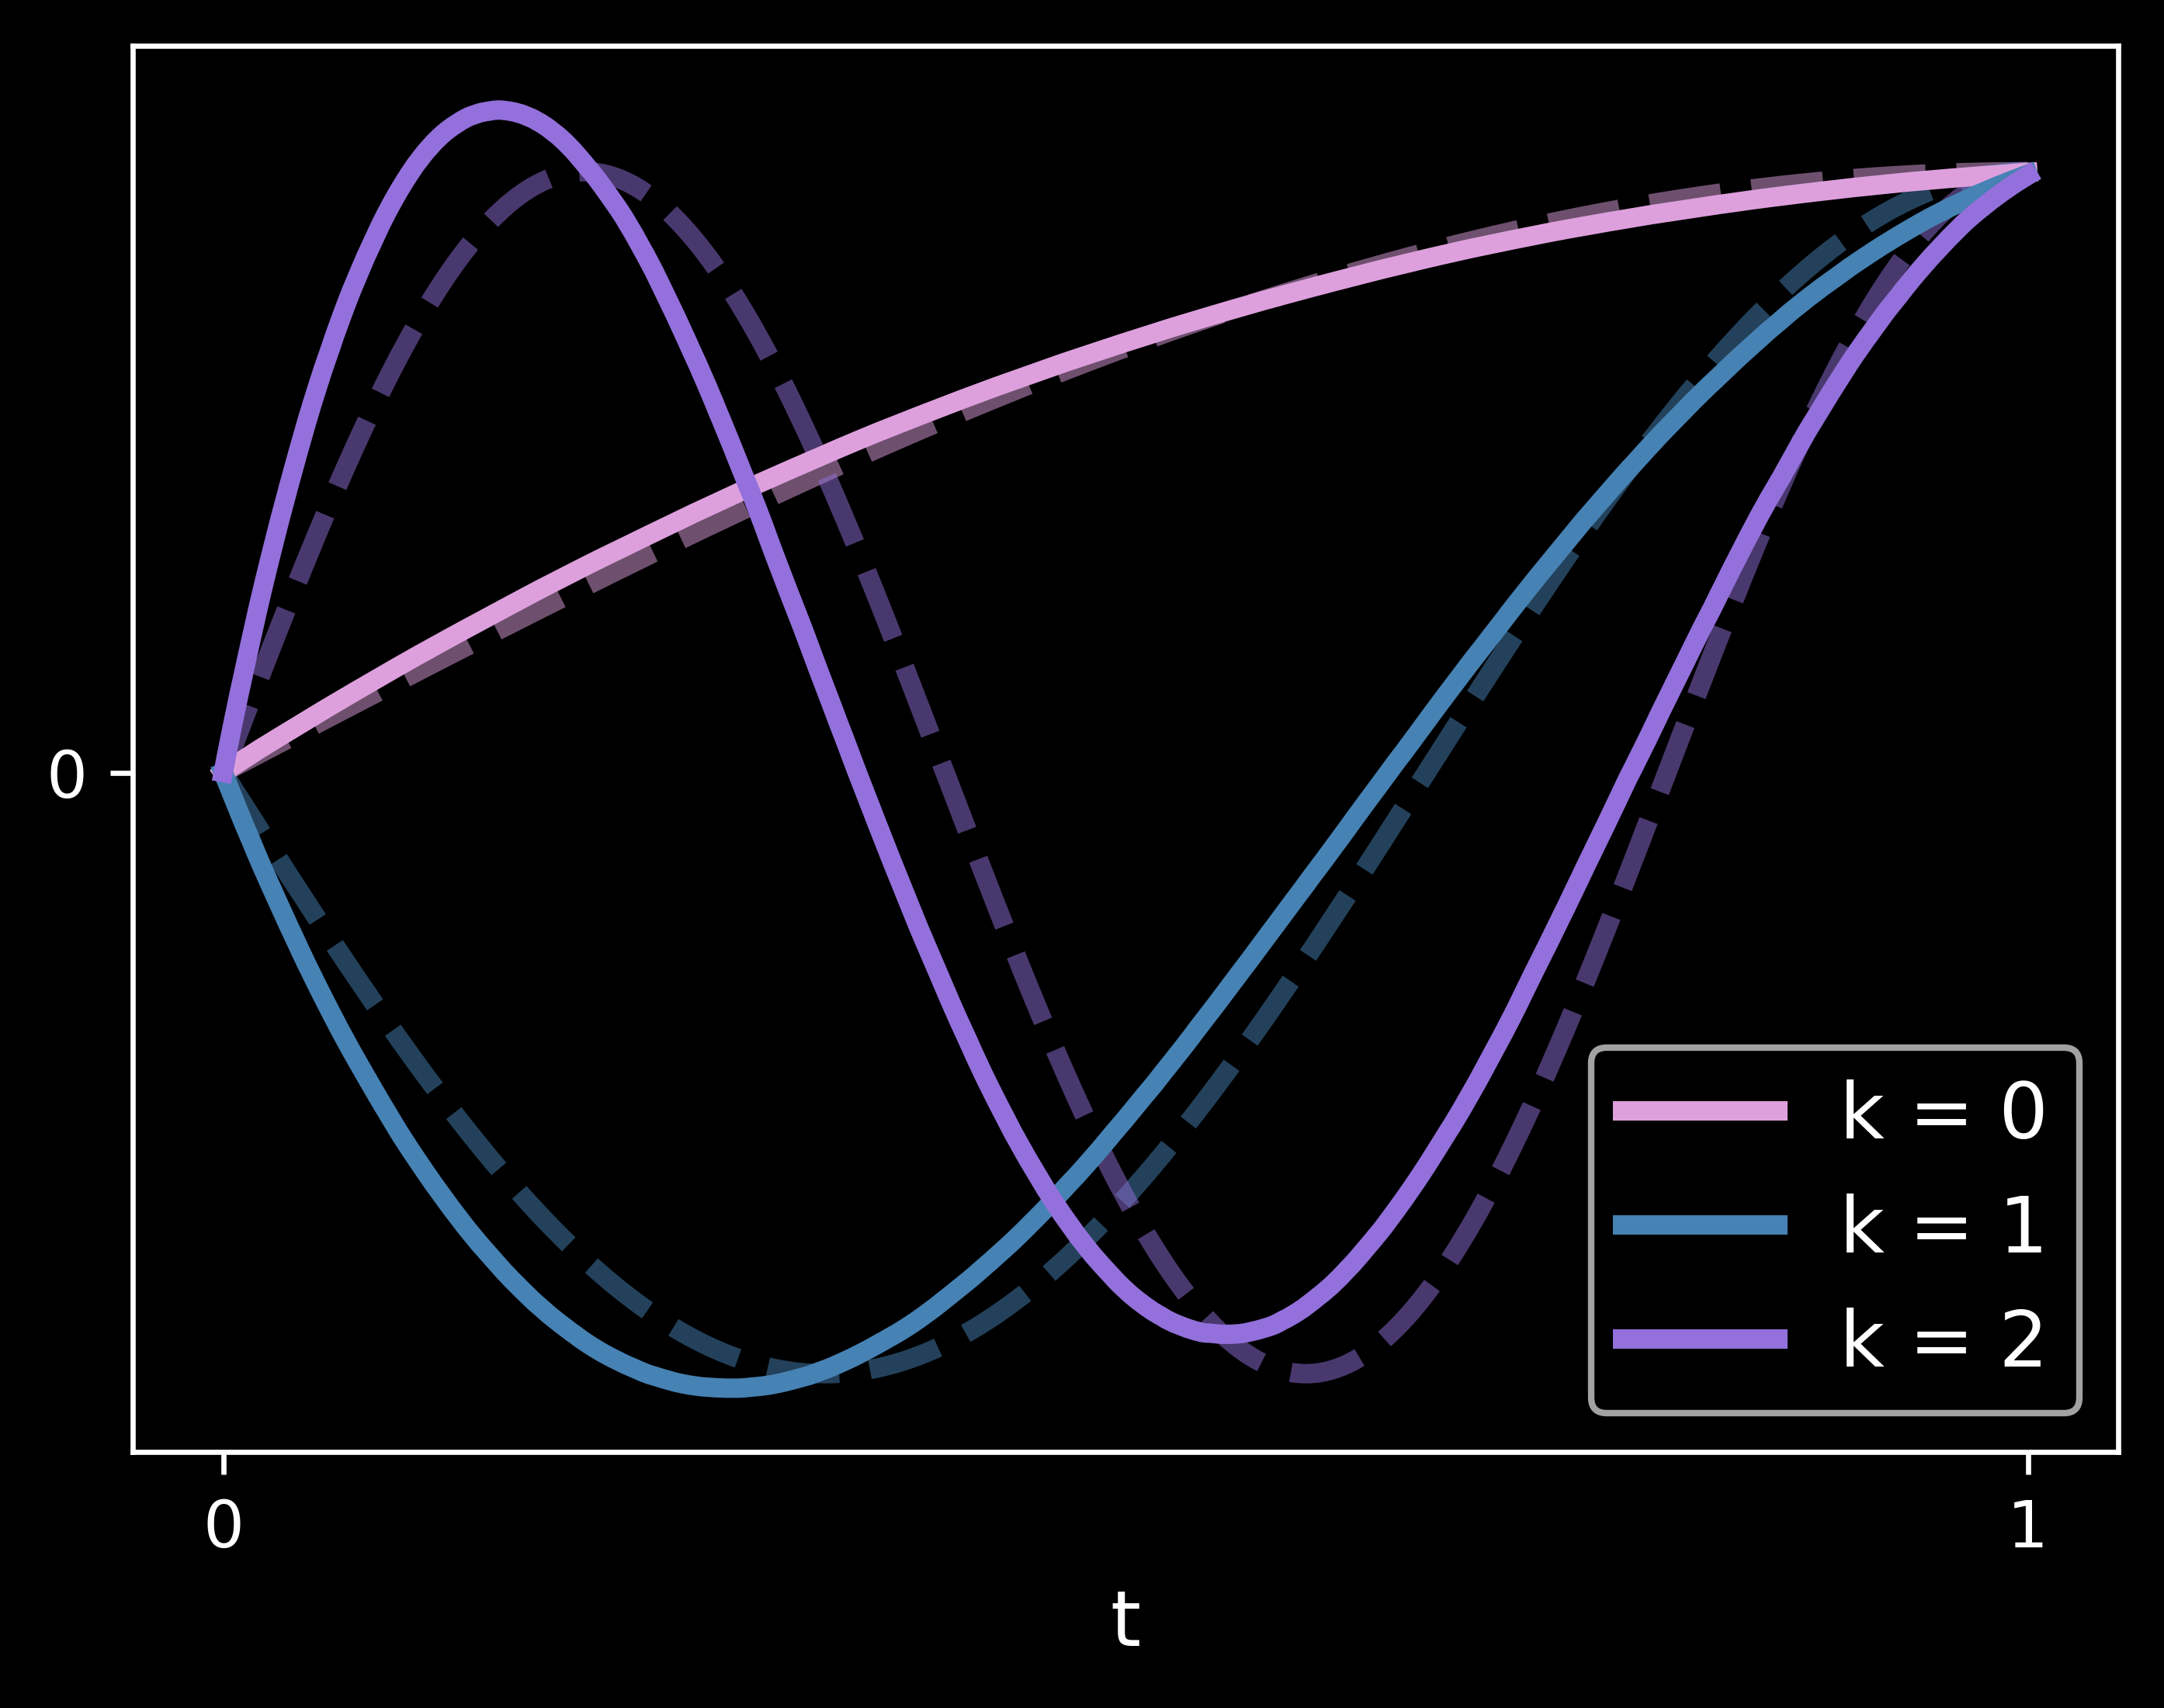
\includegraphics[scale =0.38]{KL/Figures/KLLookback.png}
\end{subfigure}
\vspace{1mm}
\begin{center}
    \footnotesize{
    \textit{Solid lines: transformed
     path.  Dashed lines: Brownian motion.}}
\end{center}
\vspace{-3mm}
\end{figure}

\subsection{Numerical Results} \label{ssec: numResult}
Let us compare the $L^2(\Q \otimes \, dt)$ error  
$\lVert Y^{K,\frakF} - Y \rVert^2_{*} $ in the Brownian case for the two avenues discussed at the beginning of this section. When $Y^{K,\frakF} = (f \circ \pi^{K,\frakF})(X) $, the error is calculated using Monte Carlo simulations. As in  \Cref{sec:numResultX}, we choose $T=1$, $N=10^4$ and $K\in \{1,\ldots,128\}$.  
\Cref{fig:L2Error} displays the result for the running maximum, integral and average functionals. We also add the Brownian motion itself, corresponding to the identity functional $f(X)=X$. We observe a clear improvement when projecting the transformed path. Moreover, it comes as no surprise that smooth functionals (integral, average) exhibits a faster rate of convergence than the running maximum, highly sensitive to local behaviours of a path. 

\begin{figure}%[H]
    \centering
    \caption{$L^2(\Q \otimes dt)$ approximation errors. }
    \vspace{-2mm}
    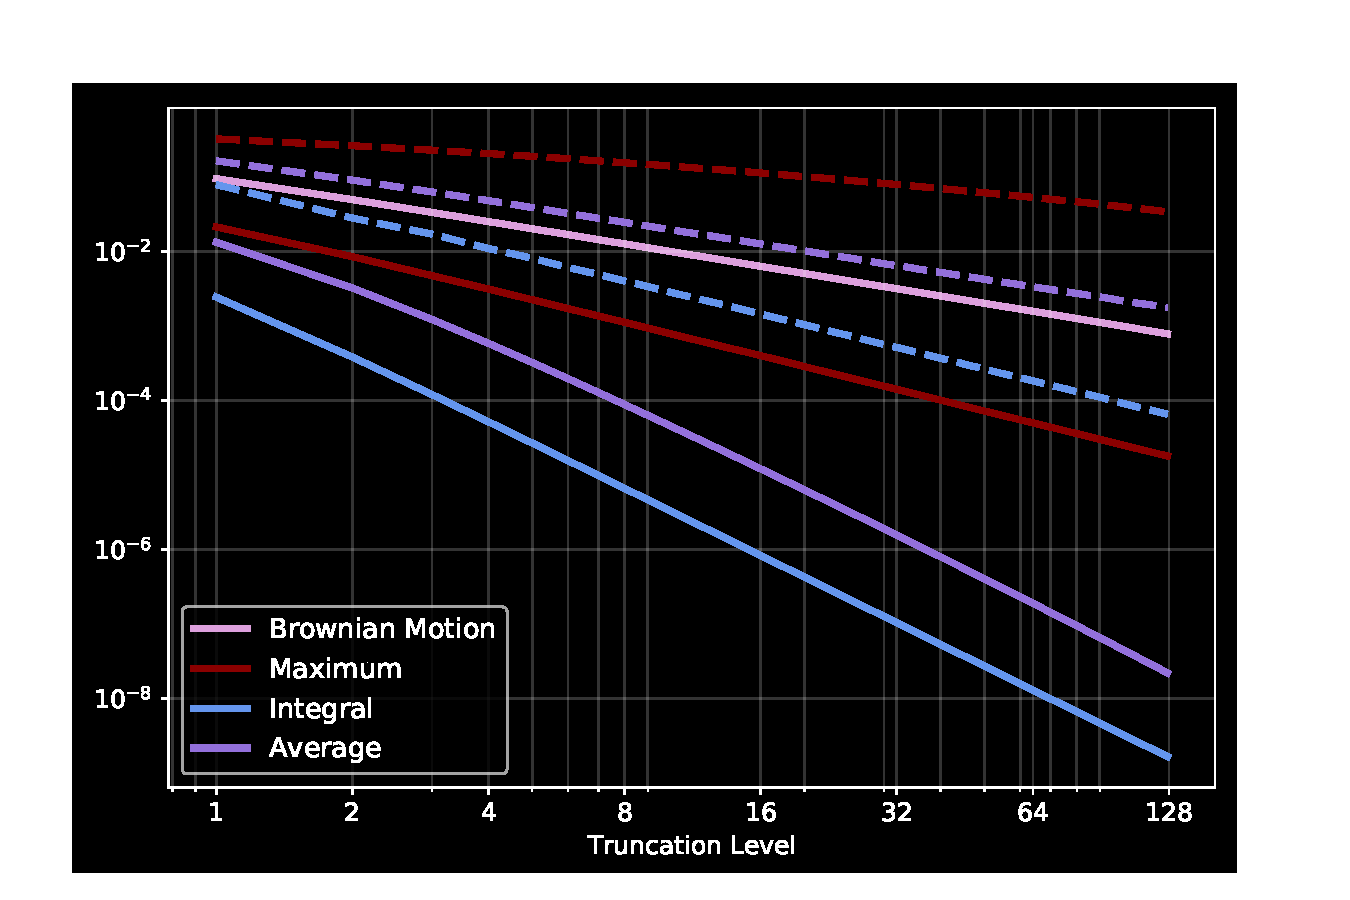
\includegraphics[scale =0.38]{KL/Figures/Error_nSim5000_N1000.pdf}
    \label{fig:L2Error}
    \\
    
    \vspace{1mm}
    
    \footnotesize{
    \textit{Dashed lines: functionals of projected paths. \\Solid lines: projected functionals.}}
\end{figure}

% \subsection{Monotone Convergence}
% When do we have $f_K \nearrow f$? This would ensure, in particular, that 
% $$\lim_{K\to \infty} \E^{\Q}[f_K(X_T)] = \E^{\Q}[f(X_T)].$$ 

% \begin{example}
% (\textbf{Running maximum}) Take 
% $f_K = f \circ \pi^{K,\frakF}$, where $\frakF$ are the Schauder functions and $\calH = \calR$. Then increasing the order $K$ adds new vertices on the graph of $x^{K,F}$ while keeping the ones already there. Hence the maximum, attained on a vertex can only increase. In other words, 
% $$f_K(X_t) = \max_{s\, \le t} x_s^{K,\frakF} = \max_{t_n\, \in \, \Pi_K} x_{t_n}^{K,\frakF} \le \max_{t_n\, \in \, \Pi_{K'}} x_{t_n}^{K',\frakF} = f_{K'}(X_t),
% $$
% if $\Pi_K$ denotes the $K-$th dyadic partition. 

% \end{example}



\subsection{Discussion: Projection of Functionals using the Signature} \label{sec:sigFunc}

Another approximation of $Y=f(X)$ can be obtained by combining  signature functionals in a linear fashion. For instance, one can consider all the words of length less than $\bar{K} \in \N$, giving the approximation
  \begin{equation}\label{eq:sigPayoff}
      y^{K,\calS}_t := \sum_{l(\alpha)\, \le \, \bar{K}} \xi^f_{\alpha} \calS_{\alpha}(X_t), 
  \end{equation}
  \vspace{-3mm}
  
  with $K = |\{\alpha \, | \, l(\alpha)\le \bar{K}\}|=2^{\bar{K}+1}-1.$
  The coefficients $\xi^f_{\alpha}$ may depend on  $X_0$  only and can be  calculated by either regressing  $Y$ against the signature elements or using a Taylor formula for functionals; see \cref{chap:Taylor}.  %\cite{LittererOberhauser} when $f$ is smooth (in the Dupire sense) and $X$ is a diffusion. 
    % In the literature,   $\eqref{eq:sigPayoff}$ is referred to  as  \textit{polynomial functional}  \cite{LittererOberhauser} or \textit{signature payoff} \cite{Szpruch,LyonsNum} in finance. 
     
     The appeal of such projection comes from the fact that polynomial functionals are dense in the space of continuous functionals restricted to  paths of bounded variation; see Theorem 5 in  \cite{LittererOberhauser}.  
     On the other hand, despite the existence of   packages to calculate the signature of discrete time paths (e.g., \texttt{iisignature} and \texttt{esig} in Python), the projection in $\eqref{eq:sigPayoff}$ is still  challenging from a computational perspective. 
     Indeed, contrary to the reconstruction in  \Cref{sec:sigLegendre}, the signature functionals have to be known at \textit{every} intermediate time. Also, as there is a priori no recipe to select words up to a given length,  we must retain all of them so the number of elements doubles every time a layer is added. 



\section{Applications} \label{sec:application}
We now illustrate the benefits of the Karhunen-Loève expansion on functionals for the pricing of exotic derivatives. % written on a single asset. 
We slightly change notations and write $W$ for the coordinate process. The path $X$ now represents the stock price where for simplicity, we employ the Black-Scholes model with zero interest rate. That is,  $\Q$ is the Wiener measure and $x_t = x_0 \calE_t(\sigma  W)$, where $x_0>0$ is fixed and  $\calE$ denotes the stochastic exponential.
Notice, however, that our method applies to any dynamics of the underlying.  

%$\varphi_m(X_t) = (f(X_t)-m\, x_0)^{+}, \, f: \Lambda \to \R,$
%where $m$ is the moneyness of the option. 
%In other words, we restrict ourselves to call options written on a path-dependent quantity of the underlying stock price.  
Let $\calM \subseteq \R$, $\calT \subseteq [0,T]$ be a finite set of option parameters and maturities, respectively. 
We seek to approximate the price surface
$p: \calM \times \calT \to \R$,  $p(m,\tau) = \E^{\Q}[ \varphi_m(X_\tau)]$, where the payoffs  $\varphi_m(X_{\tau}) = (h_m \circ  f)(X_{\tau})$ depends on a parameter $m \in \calM$.  For example, a call option on $Y=f(X)$  is obtained with $h^{\text{Call}}_m(y) := (y-m x_0)^{+}$ and $m$ is the \textit{moneyness} of the option.

The standard Monte Carlo  approach (MC) consists of simulating the underlying path  on a partition  $\Pi_{N} = \{0=t_0 < t_1 < ... < t_N=T \}$  that contains $\calT$ and compute the price as $p^{N,J}(m,\tau) = \frac{1}{J}\sum_{j=1}^J \varphi_m(X^{N,j}_\tau)$, $J\in \N$. 
In contrast, the \textit{Karhunen-Loève Monte Carlo method} (KLMC) samples $Y=f(X)$ directly and computes the price surface  using  the representation $p(m,\tau) = \E^{\Q}[ h_m(y_\tau)]$.  
We now describe the method in more depth. 
\subsection{The KLMC Algorithm}
We assume for simplicity that $Y$ has zero mean, otherwise minor changes  must be made for the KL expansion; see \cref{rem:center}. 
First, we simulate trajectories
$Y^j=(f(X_{t_n}^j))_{t_n \in \Pi_{N_{\text{off}}}}$, $j=1,...,J_{\text{off}}$ with  $J_{\text{off}}, N_{\text{off}} \in \N$,  and compute the eigenfunctions of $\kappa^{N_{\text{off}}}_Y$ as in  $\eqref{eq:eigendecomp}$. Next, for $k=1,...,K$,   we estimate the sample quantile function $\Phi_k^{-1}:[0,1]\to \R$ of $\xi_k = (Y,F_k)$ by employing method N\textsuperscript{o} $\! 7$ in \cite{HyndmanFan}.  
The coefficients $(\xi_k )$ can thereafter be simulated using inverse transform sampling \cite{Devroye}. 
  Notice that these steps can be done in an offline phase so $(\Phi_k^{-1})$ can be reused for other options contingent upon the functional $f$; see \Cref{sec:numResultX}. 
  

In the online phase, we simulate $J \in \N$ transformed paths using inverse transform sampling for $\xi_k$. This gives $y_{\tau}^{K,\frakF,j}= \sum_{k\le K}\xi_k^{j} F_k(\tau)$.  
Finally, the price surface is calculated using Monte Carlo.  The procedure is summarized in \Cref{alg:klmc}. 
It should be noted that although the coefficients $(\xi_k)$ are orthogonal in $L^2(\Q)$, they may well be \textit{dependent} when $Y$ is non-Gaussian. While the marginals of $(\xi_k)_{k\le K}$ are fitted properly, 
the dependence is omitted as generating dependent random vectors with unknown joint distribution is highly non-trivial. Nevertheless, this simplification doesn't induce a bias in the obtained prices as we shall see in the numerical experiments.  


\begin{algorithm}[t]
\caption{(KLMC) }\label{alg:klmc}
\begin{itemize}
\vspace{-2mm}
\item \textbf{Offline}: Given $f$, $K$,  $J_{\text{off}}$, $N_{\text{off}}$ 
\begin{enumerate}
\setlength \itemsep{0.2ex}
\vspace{-2mm}
\item Simulate trajectories $Y^j=(f(X_{t_n}^j))_{t_n \in \Pi_{N_{\text{off}}}}$, $j=1,...,J_{\text{off}}$
\item Compute $\kappa^{N_{\text{off}}}_Y$ (closed-form or from the sample  $(Y^j)$)
\item Solve the eigenvalue problem $\eqref{eq:eigendecomp}$ to obtain  $(\lambda^{\frakF}_k,F_k)$
\item Using $(Y^j)$, estimate the quantile functions  $\Phi_k^{-1}$, $k\le K$ 
\end{enumerate}
\vspace{-2mm}

\item \textbf{Online}: Given $J, \ \calM, \ \calT$ 
\begin{enumerate}
\setlength \itemsep{0.2ex}
\vspace{-2mm}
\item Simulate $\xi^j_k = \Phi^{-1}_k(u_k^j)$, $(u_k^j) \overset{i.i.d.}{\sim} U(0,1)$, $j \le J$, $k\le K$
\item Compute $y_\tau^{K,\frakF,j} =\sum_{k=1}^K  \xi^j_k    F_k(\tau)$, $\tau \in \calT$, $j\le J$ 
\item Estimate the price surface $p^{K,\frakF,J}(m,\tau) := \frac{1}{J}\sum_{j=1}^{J} h_m(y_\tau^{K,\frakF,j}).$
\end{enumerate}
\end{itemize}
\vspace{-3mm}
\end{algorithm}

\subsection{Numerical Results} \label{sec:numResultPrice}
First, we build the price surface for  Asian and lookback call options, i.e. by choosing $h_m = h^{\text{Call}}_m$ and the running maximum and time average as underlying functional, respectively. Of course, the put option price surface can  be retrieved thanks to  put-call parity. We also consider Up \& Out digital options, that is $f(X_t)=\max_{0\le s \le t}x_s$  and   $h^{\text{UO}}_m(y):=\mathds{1}_{\{y \ \le \ m x_0\}}$. The parameter $m\ge 1$ thus represents the barrier of the option relative to the spot price. 
We can therefore reuse the quantile functions computed for the lookback call options.

The parameters are $(x_0,\sigma,N_{\text{off}},J_{\text{off}},J) = (100, 0.2, 10^3, 2^{17}, 2^{19})$, 
 $T=1$ year and $\calT =  \{\frac{1}{52},\frac{2}{52},\ldots,1\}$ (weekly maturities). 
The moneyness and barrier levels are respectively $\calM^{\text{Call}} = \{0.75,0.80,\ldots,1.25\}$ and $\calM^{\text{UO}} = \{1.05,1.10,\ldots,1.50\}$. 
We assess  accuracy  in the mean square sense, namely by computing 
$$
\text{MSE} =  \frac{1}{|\calM|\ |\calT|}\sum_{(m,\tau) \in \calM \times \calT} |p^{\text{(B)}}(m,\tau) - \hat{p}(m,\tau)|^2. 
$$ The function $\hat{p}$ is the approximated price and $p^{\text{(B)}}$ a benchmark obtained using a standard Monte Carlo with $40 \cdot |\calT| = 2080$ time steps and same number of simulations. 
\interfootnotelinepenalty=10000 
  \cref{tab:results} displays the MSE, runtime (online phase) and number of variates per simulated path ($K$ and $N$ for the KLMC and MC method, respectively).\footnote{The experiments have been made on a personal computer; see \href{https://github.com/valentintissot/KLMC.git}{https://github.com/valentintissot/KLMC} for an implementation. The offline phase takes about 10 seconds per  functional.}  Notice that we increase $K,N$  for the lookback call and Up \& Out digital option as the running maximum has a slower rate of $L^2(\Q\otimes dt)$ convergence  as seen in \Cref{fig:L2Error} for the Brownian case.  The KLMC method constantly yields a lower MSE and runtime.  For the Asian call option, note that the number of variates per path is less than the number of maturity points and KLMC method, which couldn't be done with the MC method. 
  
 \vspace{-1mm}

\begin{table}[H]
    \centering
\caption{Mean squared errors and runtime (seconds)}
\vspace{-3mm}
\begin{tabular}{ccccccc} 
\hline  & \multicolumn{3}{c}{KLMC}  & \multicolumn{3}{c}{MC} \\  \hline
Option & K & MSE  & Time & N & MSE & Time \\
\hline  
 Asian Call & $40$ & 1.50e-04 & 2.26 & $ 52$ & 3.10e-04 & 2.40\\ 
Lookback Call   & $100$ & 1.15e-02 & 4.47& $4\cdot 52$ & 1.92e-01 & 7.05 \\ 
Up \& Out Digital   & $100$ & 1.80e-04 & 4.40 & $4\cdot 52$ & 1.90e-04 & 6.88\\ \hline
\end{tabular}
\label{tab:results}
\end{table}

\section*{Conclusion}
We shed further light on the approximation of path functionals. After a  review of Hilbert projections and a connection with the path signature, we show the power of the Karhunen-Loève expansion to parsimoniously simulate path-dependent payoffs. 
Further work would include the use of copulas in the  KLMC algorithm to capture the dependence between the $L^2([0,T])$ coefficients of the Karhunen-Loève expansion and a performance comparison with signature-based methods. 

%\bibliography{KL/ref.bib}
